\documentclass[letter,11pt]{article}

\usepackage[english]{babel}
\usepackage[T1]{fontenc}
%\usepackage[ansinew]{inputenc}
\usepackage{lmodern}	% font definition
\usepackage{verse}
\usepackage{datetime}
\usepackage{verbatim}
\usepackage{pbox}
\usepackage{float}
\usepackage{array}
\usepackage{booktabs}
\usepackage{ccaption}

\usepackage{parskip}
\usepackage{graphicx}
\usepackage[top=1.5cm,bottom=2.5cm,right=1.5cm,left=1.5cm]{geometry}
\usepackage{pdflscape}
\usepackage[numbers]{natbib}
\usepackage{minitoc}

\usepackage[urw-garamond]{mathdesign}

\usepackage{dot2texi}
\usepackage{tikz}

%%%<
%\usepackage{verbatim}
%\usepackage[active,tightpage]{preview}
%\PreviewEnvironment{tikzpicture}
%\setlength\PreviewBorder{5pt}%
%%%>

\usetikzlibrary{arrows,shapes}

\usepackage{url}
\usepackage[ps2pdf,breaklinks=true,bookmarks=true,bookmarksopen,bookmarksopenlevel=1,pdfpagelayout=OneColumn,pagebackref=true]{hyperref}
\usepackage{breakurl}
\usepackage[all]{hypcap}
\usepackage{makeidx}
\usepackage[acronym]{glossaries}

\renewcommand*{\backref}[1]{}
\renewcommand*{\backrefalt}[4]{%
  \ifcase #1 %
	  (Not cited.)%
	\or
	  (Cited on page #2.)%
	\else
	  (Cited on pages #2.)%
	\fi
}

\captionnamefont{\bfseries}
\captiontitlefont{\small}
\captiondelim{. }
\captionstyle{\centering}
\captionwidth{0.78\textwidth}
\changecaptionwidth
\precaption{\rule{0.78\textwidth}{0.4pt}\par}
\postcaption{\vspace*{1mm}\hrule}
\setlength{\abovecaptionskip}{2mm}
\setlength{\belowcaptionskip}{4mm}

\hypersetup{
    bookmarks=true,         % show bookmarks bar?
    unicode=false,          % non-Latin characters in Acrobat’s bookmarks
    pdftoolbar=false,        % show Acrobat’s toolbar?
    pdfmenubar=true,        % show Acrobat’s menu?
    pdffitwindow=true,     % window fit to page when opened
    pdfstartview={FitV},    % fits the width of the page to the window
    pdftitle={Space-TP ETIR},    % title
    pdfauthor={SU GSP10 Space Team},     % author
    pdfsubject={Space},   % subject of the document
    pdfcreator={SU GSP10 Space Team},   % creator of the document
    pdfproducer={David Dalrymple}, % producer of the document
    pdfnewwindow=true,      % links in new window
    colorlinks=true,       % false: boxed links; true: colored links
    linkcolor=blue,          % color of internal links
    citecolor=green,        % color of links to bibliography
    filecolor=magenta,      % color of file links
    urlcolor=cyan           % color of external links
}

\newcommand{\attrib}[1]{\nopagebreak{\raggedleft\footnotesize #1\par}}
\newcommand{\todo}[1]{\textcolor{lightgray}{\textit{<<#1>>}}}
\newcommand{\tbc}{\begin{center} \todo{to be completed} \end{center}}
\newcommand{\tbcsubsubsection}[1]{ \refstepcounter{subsubsection}%
  \subsubsection*{\thesubsubsection \quad #1} \tbc}
\newcommand{\newacronymd}[3]{\newglossaryentry{#1}{type=\acronymtype,name={#1},description={#2: #3},text={#1},first={#2 (#1)},plural={#1s},firstplural={#2s (#1s)}}}

\setlength{\parskip}{0.3cm plus3mm minus1mm}
\setlength{\parindent}{0cm}
\newcommand{\isp}{$I_{\rm sp}$}

%%GLOSSARY
\newacronymd{CLLSS}{Closed-Loop Life Support Systems}{are life support systems which reuse 100\% of their waste resources, with the exception of waste energy}
\newacronymd{COSPAR}{Committee on Space Research}{COSPAR promotes international scientific research in space, and provides an open forum for the disucssion of problems related to space science (for instance, organizing conferences on planetary protection policy).}
\newacronym{LEO}{LEO}{Low Earth Orbit}
\newacronymd{SSTO}{Single Stage to Orbit}{refers to a vehicle which reaches orbit without jettisoning hardware, expending only fluids. The term usually, but not exclusively, refers to reusable vehicles. \nopostdesc}
\newacronymd{ITAR}{International Traffic in Arms Regulations}{a set of United States federal regulations that restrict the international trade of items and information which is considered by the federal government to be ``munitions,'' including encryption technology and space technology}
\newacronym{ISS}{ISS}{International Space Station}
\newacronymd{ISRU}{In-Situ Resource Utilization}{refers to the usage of local resources, especially the local usage of resources found in space, as opposed to the transport of Earth resources into space or vice versa. \nopostdesc}
\newacronym{SLS}{SLS}{Selective Laser Sintering}
\newacronym{EBFF}{EBFF}{Electron Beam Freeform Fabrication}

\newglossaryentry{Isp}{text={\isp}, name={specific impulse (\isp)}, first={specific impulse (\isp)}, description={is a metric of rocket (or jet) efficiency; the change in momentum per unit amount of propellant used. (This works out to an SI unit of seconds.) The higher the specific impulse, the less propellant is needed to gain a given amount of momentum. For example, the Space Shuttle Main Engine has an \isp of 453s. \nopostdesc}}
\newglossaryentry{gyrotron}{text={gyrotron}, name={gyrotron}, description={a type of high-powered microwave transmitter}}

\newglossaryentry{payload-fraction}{name={payload fraction},description={the fraction of a launch
vehicle's mass on the launchpad which is allocated to the object(s) being
launched (payload), rather than structural materials, fuel, etc. \nopostdesc}}

\newglossaryentry{rocket-equation}{name={ideal rocket equation},description={an equation which relates
the maximum change of speed of a rocket with the \isp and the initial and final mass of the rocket.
\[\Delta v = I_{\rm sp} g_0 \ln \frac{m_0}{m_1}\] where $m_0$ is the initial total mass, including
propellant; $m_1$ is the final total mass, \isp is the specific impulse of the engine, $g_0$ is the
initial acceleration due to gravity, and $\Delta v$ is the change of speed of the rocket over the
entire period}}

\glossarystyle{list}
\makeglossaries
% rubber: rules rubber.ini
% rubber: onchange etir.glo '''makeglossaries etir'''
% rubber: watch etir.glo
% rubber: depend etir.glo
% rubber: clean etir.glg
% rubber: clean etir.glo
% rubber: clean etir.gls
% rubber: clean etir.ist
% rubber: clean etir.out
% rubber: clean etir.tdo
%%END GLOSSARY

\makeindex

\begin{document}

%%TITLE PAGE
\thispagestyle{empty}
\pdfbookmark[1]{Title Page}{titlepage}
\begin{tikzpicture}[overlay,remember picture]
	\node[yshift=0.5cm] at (current page.center) { 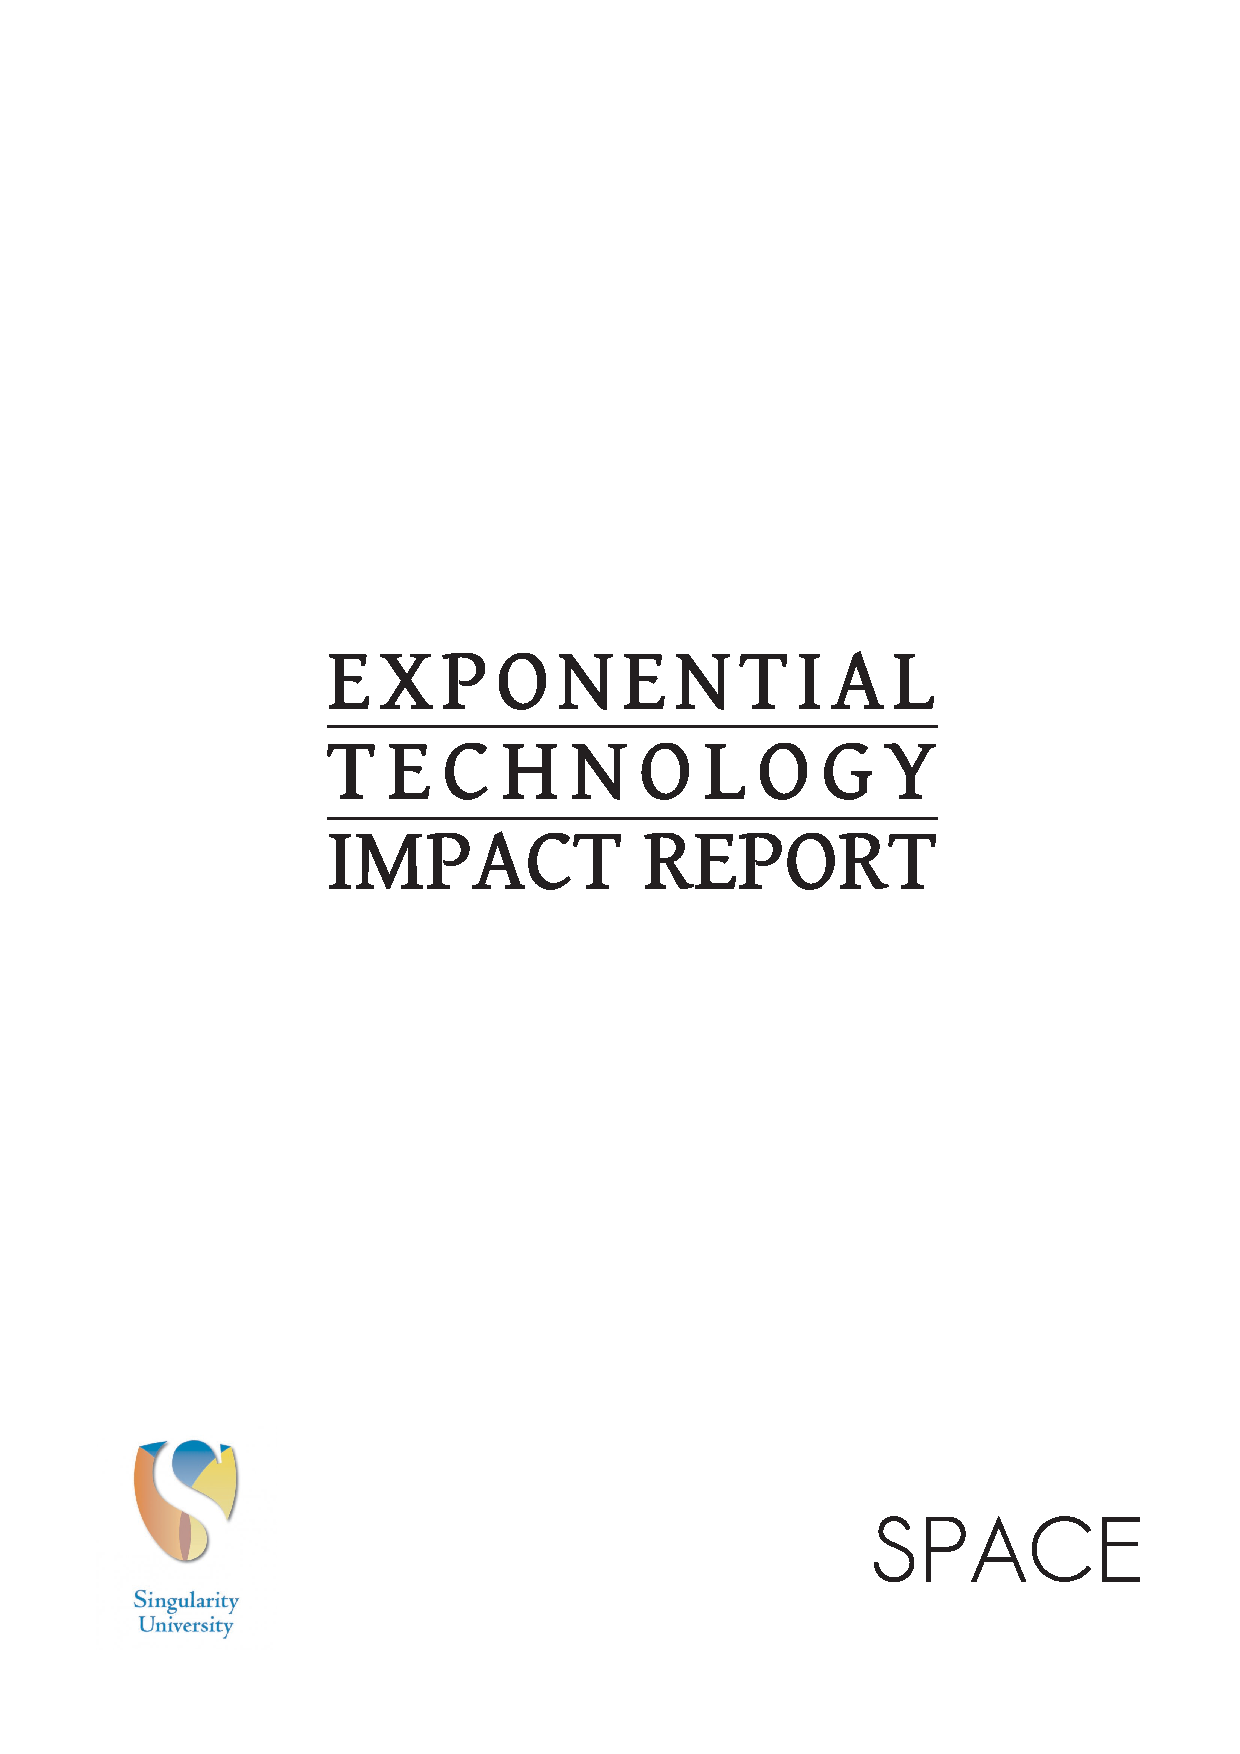
\includegraphics{etir-page1} };
	\node[yshift=-0.7cm] at (current page.center) { \huge version 0.foobar };
	\node[yshift=-1.6cm] at (current page.center) { \LARGE \today \hspace{0.2cm} \currenttime };
	\node[yshift=0.2cm] at (current page.center) { \huge \color{red!70!white} \em DRAFT };
\end{tikzpicture}

%%TABLE OF CONTENTS
\newpage
\pdfbookmark[1]{Table of Contents}{contents}
\dosecttoc
\renewcommand{\stctitle}{Contents of this Section}
\tableofcontents

\newpage

%%SUBSTANCE BEGINS HERE
\section{Scope of this Report}

\vspace{15pt}
\settowidth{\versewidth}{The surface of the earth is the shore}
\begin{verse}[\versewidth]
	\begin{altverse}
		\em
		The surface of the Earth \\
		is the shore of the cosmic ocean \\
		Recently we've waded a little way up \\
		and the water seems inviting \\
	\end{altverse}
\end{verse}
\attrib{\textbf{-- Carl Sagan\index{Sagan, Carl}}, \textit{``A Glorious Dawn''}}
\vspace{20pt}

Humanity is presently a one-planet species. Although we have sent
humans into space, and even to the moon, they have only visited and
then returned home to Earth. There are two ways in which this
fundamentally limits us: First, it limits the resources available to
us, in terms of both matter and energy. Second, it makes us vulnerable
to total destruction as a species, should a catastrophe of planetary
scale occur.

This report focuses on applications of exponential technologies that may
facilitate the eventual establishment of a permanent human presence in space.
These steps include the development of technologies to reduce the barriers to
entry into space, technologies that may be needed to remain in space
indefinitely (while also being useful on Earth), practical strategies to use
resources which are off Earth, transformative changes in the business of space
science and exploration, and means to educate, excite, and inspire the general
public about the possibilities and importance of human space exploration.

\subsection{Structure of this Report}

\todo{TODO: Graphical diagram explaining structure of final report}

\todo{This part of the document is under heavy construction. This is the temporary home of the digraph.}

\subsubsection{Digraph}

\todo{This is incomplete, represents scope}

\todo{Example about how to parse this graph---narrative threads run bottom-to-top}

\begin{landscape}
\begin{tikzpicture}[scale=0.28,>=stealth]
	\begin{scope}
	\tikzstyle{stdbox} = [draw,shape=rectangle,minimum size=1em,inner xsep=0.25em,inner ysep=0.25em,font=\tiny,text badly centered];
	\tikzstyle{emph} = [font=\tiny\bfseries,thick];
	\colorlet{challenge}{red}
	\colorlet{exptech}{green}
	\tikzstyle{challenge} = [stdbox,draw=challenge,emph,fill=challenge!50];
	\tikzstyle{exptech} = [stdbox,draw=exptech,emph,fill=exptech!50];
\begin{dot2tex}[codeonly,dot,tikz]
digraph G {
  ratio=0.7;
	rankdir=BT;
	//% GRAND CHALLENGES
	node [style="challenge"];
	getting_there [label="Getting There"];
	staying_there [label="Staying There"];
	human_exploration [label="Human Exploration",style="challenge"];
	resources [label="Space Resources"];
	robotic_exploration [label="Robotic Exploration",style="challenge"];
	science [label="Space Science"];
	education [label="Space Evangelism"];
	backup [label="Insuring Humanity"];

	edge [style="thick,color=challenge"];
	human_exploration -> staying_there; //[dir="none"];
	robotic_exploration -> science;
	robotic_exploration -> resources;
	staying_there -> backup; //[dir="none"];

	edge [style="semithick,color=challenge"];
	resources -> staying_there; //[dir="none"];
  getting_there -> resources;
	human_exploration -> science; //[dir="none"];
	getting_there -> education;
	getting_there -> robotic_exploration;
	getting_there -> human_exploration;

  //% EXPONENTIAL TECHNOLOGIES
	node [style="exptech"];
	nano [label="Nanotechnology"];
	bio [label="Biotechnology"];
	neuro [label="Neurotechnology"];
	ai [label="AI & Robotics"];
	computing [label="Networks & Computing"];

	edge [style="thick,color=exptech"];
	computing -> ai;
	neuro -> ai [dir="both"];
	computing -> bio;
	ai -> bio;
	bio -> nano [dir="both"];
	bio -> neuro;
	nano -> computing;

  node [texmode="raw",style="stdbox"];
	edge [style=semithick];
  cats [label="CATS"]
	cats -> getting_there;
	cats -> education;
	//% beam_power [label="Beam Power"];
	//% beam_power -> cats;
	//% heat_exchanger -> beam_power;
	//% heat_exchanger [label="Heat Exchanger"];
	structural_materials [label="Structural Materials"];
	thermal_materials [label="Thermal Materials"];
	nano -> thermal_materials;
	nano -> structural_materials;
	//% thermal_materials -> heat_exchanger;
	stirling [label="Stirling Engine"];
	thermal_materials -> stirling;
	energy [label="Space Energy"];
	stirling -> energy;
	energy -> resources;
	pv [label="Photovoltaics"];
	sbsp [label="\pbox{2.5cm}{Space-Based Solar Power}"];
	sbsp -> energy;
	pv -> sbsp;
	nano -> pv;
  structural_materials -> light_lv;
	light_lv [label="Lighter Launch Vehicles",style="stdbox,text width=2.4cm"];
	light_lv -> cats;
	//% light_lv -> ssto;
	//% ssto [label="Single-Stage to Orbit"];
  //% ssto -> cats;

	//% psychmon [label="Psych. Monitoring"];
	//% neuro -> psychmon;
	//% psychmon -> human_exploration;
	rubisco [label="RubisCO"];
	bio -> rubisco;
	terraforming [label="Terraforming"];
	rubisco -> terraforming
	terraforming -> staying_there

	suit [label="Nanotech Space Suits"];
	nano -> suit;
	suit -> human_exploration;

	asteroid_mining [label="Asteroid Mining"];
	asteroid_mining -> resources;
	cats -> asteroid_mining;
	//% metal_digesters [label="Metal Digesters?"];
	//% bio -> metal_digesters;
	//% metal_digesters -> asteroid_mining;

	aisyn [label="AI\&SynBio"];
	ai -> aisyn;
	bio -> aisyn;
	aisyn -> terraforming;
	human_enhancement [label="Human Enhancement"];
	aisyn -> human_enhancement;
	brain_simulation [label="Brain Simulation"];
	neuro -> brain_simulation;
	brain_simulation -> human_exploration;
	brain_simulation -> robotic_exploration;
	human_enhancement -> human_exploration;
	life_support [label="Life Support"];
	aisyn -> life_support;
	life_support -> human_exploration;
	life_support -> staying_there;

	bmi [label="Brain-Machine Interface"];
	neuro -> bmi;
	bmi -> robotic_exploration;
	bmi -> human_exploration;

	bio_research [label="Bio Research in $\mu$Gravity"];
	bio -> bio_research;
	bio_research -> science;

	neuro_treat [label="Neurotech Treatments"];
	neuro_treat -> human_exploration;
	neuro -> neuro_treat;

	space_portal [label="Space Portal/VR"];
	computing -> space_portal;
	ai -> space_portal;
	space_portal -> education;

	astro_bot [label="Companion Robot"];
	ai -> astro_bot;
	astro_bot -> human_exploration;

	microbe_fuel [label="Microbial Fuel Cells"];
	microbe_fuel -> life_support;
	bio -> microbe_fuel;

	print [label="3D Printing"];
  computing -> print;
	nano -> print;
	print -> asteroid_mining;
	print -> cats;

	bio_rad [label="Biopolymer Radiation Shield"];
	bio -> bio_rad;
	bio_rad -> human_exploration;

	space_comp [label="Space Supercomputer"];
	computing -> space_comp;
	space_comp -> ipip [dir="both"];
	space_comp -> resources;

	swarm [label="Swarms"];
	ipip -> swarm;
	swarm -> space_comp;
	swarm -> cats;
	swarm -> robotic_exploration;

	auto_explore [label="Autonomous Explorers",style="stdbox"];
	ai -> auto_explore;
	auto_explore -> robotic_exploration;
	auto_explore -> asteroid_mining;

	ipip [label="Interplanetary Internet"];
	computing -> ipip;
	ipip -> auto_explore;
	ipip -> robotic_exploration;

	spider_silk [label="Spider Silk"];
	spider_silk -> structural_materials;
	bio -> spider_silk;
	bioreactors [label="Bioreactors"];
	bioreactors -> life_support;
	bio -> bioreactors;
}
\end{dot2tex}
\end{scope}
\end{tikzpicture}
\end{landscape}




\section{Aspects of the Problem Space}
% Short description of the entire Problem Space
Doing business in space should be easy, but it isn't. It's hard to get into
space, even sending robots rather than humans. It's hard to stay in space for
very long--again, even if you send robots.  It's hard to make use of the
resources available in space. And it's hard to convince many people that going
to space is even a good idea.
% TODO?

We have chosen to focus on the following aspects of the problem space:
%Detailed description of aspects of the problem space

\subsection{Getting There}
%(to be written by Dmitriy)

The key problem driving the cost of space access today is fundamental
inefficiency of chemical rockets. In the year 2010 payloads are delivered into
orbit the same way they were launched in 1960s: by exploding large amounts of
chemicals in a semi-controlled way. Conventional multistage rockets are limited
to \glspl{payload-fraction} of less than 4\%. Using the \gls{rocket-equation},
it is easy to see that this inefficiency is caused partly by the structural
limits of existing materials, and partly by the limited \gls{Isp} of chemical
propellants, which have reached a practical limit of 453 seconds. 
 
Inefficiency of chemical propulsion results in unreasonable complexity of
present day launch vehicles, which operate on the very limits of structural
margins. This requires a large number of people to work on the maintenance,
operation and pre-flight checks.  It also prevents reusability of rockets,
leading to unacceptably high risks associated with launch and extremely high
costs of payload insurance. Launch of a chemical rocket is a violent process
and a structure operating near its design tolerance is more susceptible to
fatigue and failure. The Space Shuttle, as a reusable vehicle, requires
extensive refurbishment and safety checks between launches, to the extent that
the launcher is disassembled, inspected, refurbished and rebuilt before every
launch. For example, a hydrogen tank used for the on-board fuel cell is
manufactured to burst at 1.5 times its usual operating pressure in order to
save mass, but this safety factor of 1.5 means the tank may last only 100
cycles. Such a failure-prone component must have a more regular inspection
regime, so operational costs go up. In contrast, the fuselage of a pressurized
civil aircraft has a safety factor of two, and for that relatively little extra
mass will last tens of thousands of pressurization cycles. 
 
The high cost of space launch arises not only from technical challenges but
also from the absence of economic incentives and the lack of a well defined
market.  Although, we would argue, those economical challenges will be
eliminated as soon as the technical challenges of building cheap and reliable
launch vehicles are resolved. On the economic side, various market models
predict an essentially flat elasticity of demand for space access until the
cost of launch is reduced below \$1000 per kilogram\cite{CommSpace1997}. (See
\autoref{launch-cost}.) This implies that the primary economic benefits of space
cannot be realized without an order of magnitude reduction in launch costs and
hence, without a paradigm shift in the means of space launch systems. 
 
\begin{figure}[bt!]
	\centering
	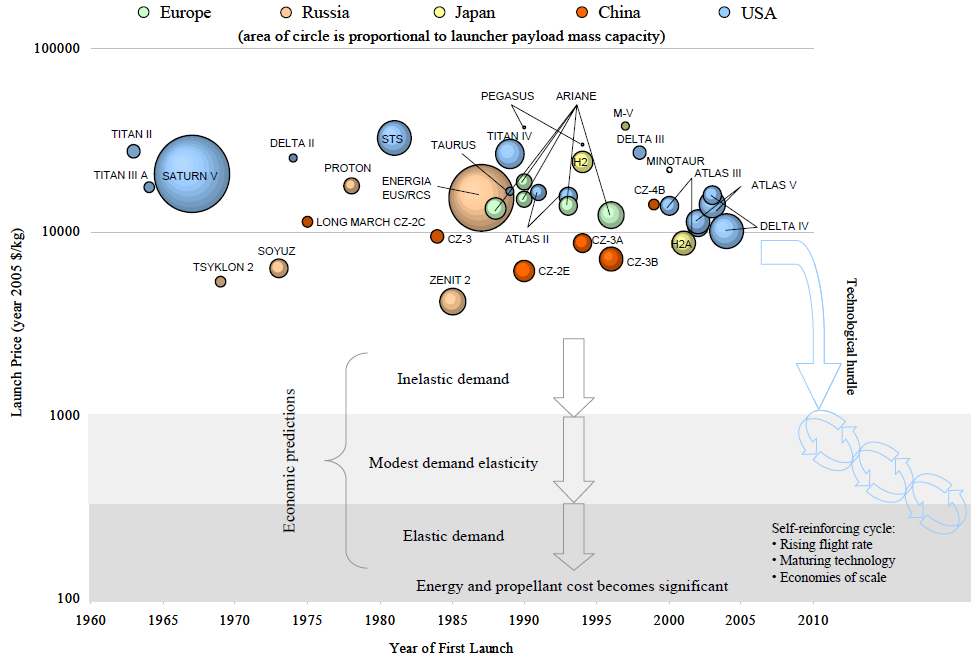
\includegraphics[width=\textwidth]{launch-cost}
	\caption{Cost of space access over the last 5 decades}
	\label{launch-cost}
\end{figure}

An additional problem that is deeply rooted in the inefficiency of chemical
rockets and the absence of mature space exploration market is lack of mass
produced cheap components for space launch systems. All critical components are
custom produced and tested by large teams over long periods of time. This leads
into yet another problem: the time lags between the payload production and
launch are unacceptably long and can hardly fit into business models of small-
and medium-sized businesses which demand expediency as they are driven by the
demand of rapid growth. Moreover, the current way of space transportation often
requires high level of integration between the launch vehicle and the payload,
which means that the customer is forced to choose the supplier long in advance
and coordinate the development of payload with the launch provider. 

In summary, launch is currently almost prohibitively expensive, infrequent, and
inconvenient. Any transformative change in the landscape of space activity will
require more effective launch systems.

\subsection{Staying There \label{staying-there}}

The conditions we have to create in space for human life to thrive are to some
extent the same humans need to create in order to stay on Earth. As we need to
create conditions on Earth which are conducive to life, so have we in space.
However, between the two environments there are some fundamental differences.
In space the key challenges derive from: lack of breathable air/atmosphere;
lack of all other life support systems, services, and goods/materials provided
on Earth by Nature, as well as extreme temperatures; radiation; absence of or
reduced gravity; different light-dark patterns; reduced number of people, at
least in the early stages of space colonization, isolation, and reduced
availability of physical space.
 
A space system inhabitable by humans, at least given present technologies,
should be designed in order to become, at a certain point, closed for matter
and open for energy. All the living parts and beings would be interconnected
and interdependent, as well as diverse and symbiotic.
 
Staying in a space environment, either grounded or ungrounded, requires the
respect of three fundamental principles: 
 
\begin{enumerate}

	\item     People in the space environment should not be subject to increasing
		concentrations of substances produced by human activity, such as molecules
		or chemical substances which if not removed would accumulate in air, soil,
		water, or other materials (for example CO$_2$, CH$_4$, other chemical
		substances).

	\item     In a thriving space environment the fundamental life support
		systems should be recreated and operated in a reliable way, indefinitely in
		time. Through photosynthesis, or other processes achieving a similar
		result, the space life-support systems should be able to regenerate order
		and structure for human use, starting from higher levels of disorder, using
		external energy sources.

 \item     In space settlements people should not subject to conditions that
	 systematically compromise their capacity to satisfy their fundamental human
	 needs. Human needs can be classified in nine categories, in four domains---%
	 Being (qualities), Having (things),  Doing (actions), Interacting (settings)%
	 ---and all should be satisfied for a healthy and thriving life:

\begin{center}
  \small
	\begin{tabular}{>{\centering\bfseries}m{0.17\textwidth}*{4}{>{\centering}m{0.16\textwidth}}}
		\textsc{Fundamental Human Needs} & \bfseries Being & \bfseries Having & \bfseries Doing & \bfseries Interacting \tabularnewline\toprule
subsistence &
physical and mental health &
food, shelter, work &
feed, clothe, rest, work &
living environment, social setting \tabularnewline\midrule
protection &
care, adaptability, autonomy &
social security, health systems, work &
co-operate, plan, take care of, help &
social environment, dwelling \tabularnewline\midrule
affection &
respect, sense of humour, generosity, sensuality &
friendships, family, relationships with nature &
share, take care of, make love, express emotions &
privacy, intimate spaces of togetherness \tabularnewline\midrule
understanding &
critical capacity, curiosity, intuition &
literature, teachers, policies, educational &
analyse, study, meditate, investigate &
schools, families, universities, communities \tabularnewline\midrule
participation &
receptiveness, dedication, sense of humour &
responsibilities, duties, work, rights &
cooperate, dissent, express opinions &
associations, parties, churches, neighborhoods \tabularnewline\midrule
leisure         &
imagination, tranquillity, spontaneity  &
games, parties, peace of mind &
day-dream, remember, relax, have fun &
landscapes, intimate spaces, places to be alone \tabularnewline\midrule
creation &
imagination, boldness, inventiveness, curiosity &
abilities, skills, work, techniques &
invent, build, design, work, compose, interpret &
spaces for expression, workshops, audiences \tabularnewline\midrule
identity &
sense of belonging, self-esteem, consistency &
language, religions, work, customs, values, norms &
get to know oneself, grow, commit oneself &
places one belongs to, everyday settings \tabularnewline\midrule
freedom &
autonomy, passion, self-esteem, open-mindedness  &
equal rights &
dissent, choose, run risks, develop awareness &
anywhere \tabularnewline\midrule
\end{tabular}
\end{center}
\end{enumerate}
 
If humans in space should be deprived of the capacity to satisfy any of the
needs above, in a sufficiently abrupt manner or for a sufficiently long time
duration, they would face a mental and/or physical poverty at first, and
eventually, if the deprivation persists, they could be led to death. Any
relational or governance system established in a space environment, especially
with the goal of ``staying there,'' should consider all the fundamental human
needs above. It should be noticed that while the satisfiers of the needs change
across cultures, or time, the needs themselves remain constant. For this
reason, a space environment and space activities should be designed to maximize
the satisfaction of the human needs without violating the previous principles.
This result can often be conveniently achieved through dematerialization, which
becomes more and more effective with the advancement of exponential
technologies such as augmented virtual reality. The fundamental design
principles for human interaction in space could be the ``Golden Rule'': ``Would
I like to be subject to such conditions I am creating?''

Once the design principles above have been considered, the challenge remains
how to implement them in the extreme space environment.

\begin{comment}
 REFERENCES:
 Fundamental Human Needs: \url{http://en.wikipedia.org/wiki/Fundamental_human_needs}
 Design principles: \url{http://www.naturalstep.org/sites/all/files/Strategic_SD_0.pdf}
 
Colonization of the Moon, Mars, and Other Planets
 
\url{http://settlement.arc.nasa.gov/}
 
\url{http://nssdc.gsfc.nasa.gov/planetary/mars/mars_colonize_terraform.html}
 
\url{http://www.washingtonpost.com/wp-dyn/content/article/2005/09/23/AR2005092301691.html}
 
\url{http://www.hq.nasa.gov/office/hqlibrary/pathfinders/colony.htm}
\end{comment}


\subsection{Human Exploration}
%(to be written by Sarah Jane)

%emailed

Human exploration beyond Earth's atmosphere presents many threats and promises
to meeting basic human needs: The conditions are inhospitable to human life.
There is no known air source. The temperatures are extreme. Radiation is
intense. Meteor showers, solar flares, debris and dust are ever-present
threats. Human--rated infrastructures and outposts do not exist. Other forms of
life have yet to be found.  The challenges associated with understanding and
preparing for optimum general human wellbeing in space is multitudinous. The
recommendation, risk assessment and mitigation (be it technology,
countermeasure development or advanced life supports and protocols) for the
enhanced well being, performance, operation and happiness of the crews is
imperative.

\subsubsection*{Closed Loop Life Support Systems (CLLSS)}

The CLLSS components, resources and technologies needed to provide a basic foundation for a live-able, controllable and recoverable environment for human space flight and habitability must include the following space-rated systems:

\begin{itemize}
	\item Atmospheric Revitalization

	\item  Water Recovery

  \item Waste Management

  \item Habitation System

  \item Environmental Monitoring

  \item Pressure Control

  \item Fire Protection

  \item Thermal Control

\end{itemize}

NASA's ECLASS can only achieve a 65\% closed loop effectiveness with current
systems technology (\autoref{eclss65}). This is acceptable for short duration
human space flight and life onboard the \gls{ISS}, but it does not suffice for
further human exploration.

 
\begin{figure}[hb!]
	\centering
	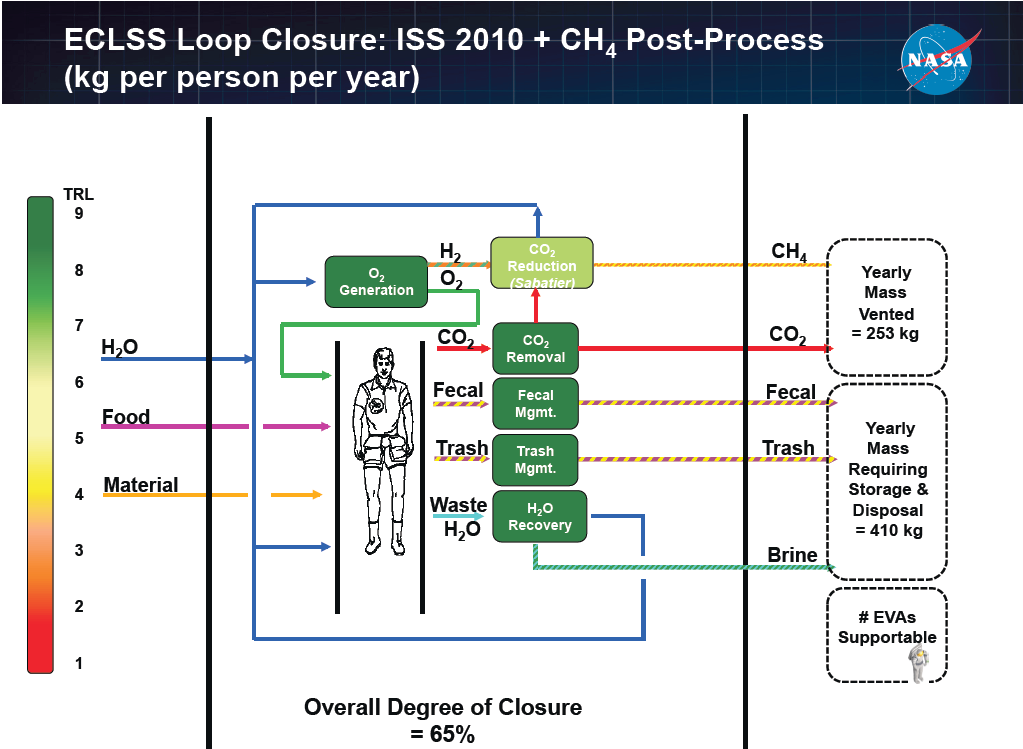
\includegraphics[width=\textwidth]{SJTable1}

	\caption{ECLSS Loop Closure: ISS 2010 + CH$_4$ Post-Process (kg pp/py) = 65\% effectiveness \cite{Neumeyer2010}}
	\label{eclss65}
\end{figure}

\begin{description}
\item[Food:] Need for a way to generate a complete, well rounded diet with minimal
input and output, 100\% closed loop if possible.  Bonus: enjoyable to eat.

\item[Water:] Need: Sophisticated waste and grey water systems to allow for closed loop water systems.

\item[Waste:] Design waste out of the system. Design and engineer systems able to operate completely in loops closed for matter and open for energy.

\item[Air:] Assure fully recyclable air systems able to work indefinitely at 100\% reliability.
\end{description}

Reliable fully closed loop life support systems for humans (\autoref{eclss95})
need to be demonstrated in ground test facilities and in space with increased
performance efficiencies such that little-to-no-maintenance, re-supply and the
capacity for bio-regeneration is incorporated into the design metrics towards
future autonomous space system adaptation and in situ resource utilization. We
must advance, demonstrate, and integrate current space rated hardware with new
technologies and strategies to also reduce the mass, power and re-supply
requirements when measured against the current state of the art space flight
qualified hardware and work towards both the issues of human survivability and
longevity whilst in space.
 
\begin{figure}[hb!]
	\centering
	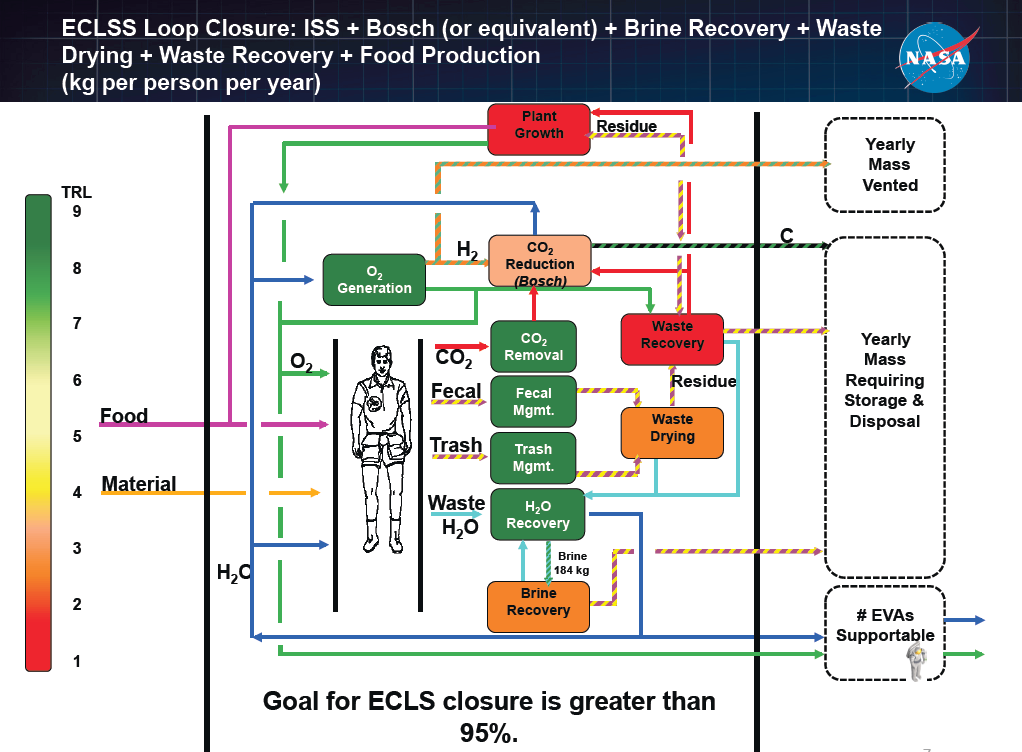
\includegraphics[width=\textwidth]{SJTable2}

	\caption{ECLSS Loop Closure: ISS + Bosch (or equivalent) + Brine Recovery + Waste Drying + Waste Recovery + Food Production (kg pp/yr) = 95\% effectiveness \cite{Neumeyer2010}}
	\label{eclss95}
\end{figure}

\begin{comment}
Added to BibTeX	
	NASA Flagship Technology Demonstrator (FTD) Environment Control & Life Support (ECLS) Enterprise Workshop, Derek Neumeyer 2010 http://www.nasa.gov/pdf/458815main_FTD_EnvironmentControlAndLifeSupport.pdf
\end{comment}

\subsubsection*{Human Factors}

Extreme environment architectures and habitat design greatly impact human
performance, behaviors and limits in everyday life as equally as instances of
great stress. As we know it, life in the space environment presents many
challenging factors for the crew including: conditions of prolonged
confinement, isolation, information saturation, performance pressure, constant
monitoring, time delays, unnatural lighting, limited color palette and seasonal
change, limited personal space, restricted access, thermal difference, the
reliance on reconstituted air, water, tactile starvation and increasing
physical acclimation as a result of radiation and microgravity. Reliability and
diversity are equal yet opposite needs for optimum human habitat design in
extreme environments.

\subsubsection*{Extreme Design}

Human-rated structures and habitable architectures for use in extreme
environments such as space must satisfy very unique requirements. Temperature
extremes, gravity, shielding from solar and cosmic radiation and
micro-meteoroid impacts, vacuum / internal pressurization, abrasive and toxic
materials such as planetary dust must be factored into design requirements.
These issues pose great challenges to the structural adequacy, materials
science and maintenance, compatibility, functionality, access and cost of
suitable architectures and structures.

 
\subsubsection*{Physiological Health}

Physiological acclimation in space flight is complex and diverse involving
multiple systems (\autoref{acc-timeline}). Past, present and future
countermeasures in space flight require ongoing and additional review. Evidence
of $\mu$gravity-induced physiological acclimation is known. Evaluations on
crews in space analogue environments, space flight and \gls{ISS} flights are
ongoing yet the long term effects yet to be fully known and mitigated. Medical
risks variable and the delivery of medical interventions, preventions and care
needs to be refined.  The effects of microgravity and radiation are the most
problematic to human exploration in space. For instance, reliable and suitable
materials technology, design and mitigation for radiation are needed.
Acceptable radiation exposure limits need to be established. Alert/warning and
communications infrastructure from pre-screening, to initial construction
through to settlement phases need to be formalized to analyze the long-term
health risks. Microgravity (from muscle atrophy, vestibular and ocular
disturbance, venous pooling to sleep disturbance and sanitation issues) have
been evidenced and greatly impact crew performance, health and well being, thus
impacting on the entire mission.
 
\begin{figure}[hbt!]
	\centering
	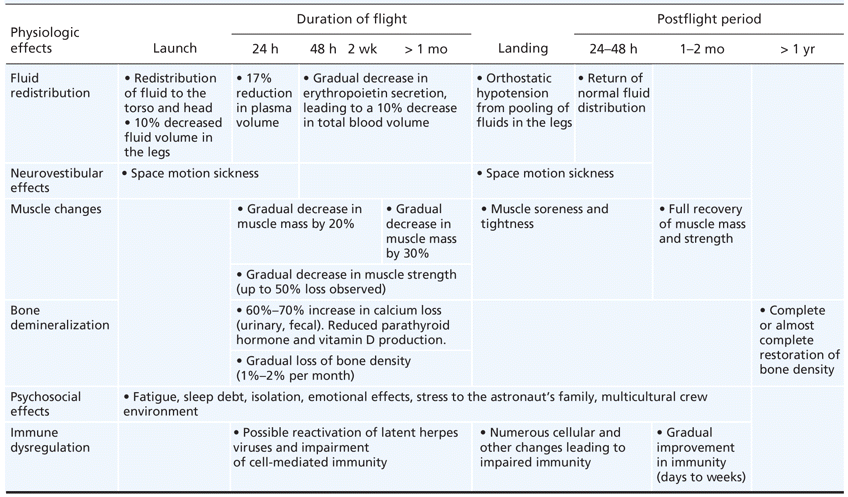
\includegraphics[width=\textwidth]{SJTable3}

\caption{Timeline of physiologic acclimation and acclimatization experienced by astronauts from launch to after return to earth\cite{Williams2009}}
  \label{acc-timeline}
\end{figure}

Other problems include \begin{enumerate} \item Bone demineralization leading to space-related osteoporosis and vitamin loss \item Temperature extremes \item Circadian dysynchrony and sleep disturbance \item High vacuum (decompression illness) \item Space debris \item Ionospheric plasma and \item Acoustic noise \end{enumerate}

\begin{comment}
Added to BibTeX
Ref:"Acclimation during space flight: effects on human physiology", David Williams, MDCM MSc, Andre Kuipers, MD, Chiaki Mukai, MD PhD andRobert Thirsk, MDCM SM. CMAJ • June 23, 2009; 180 (13). First published June 9, 2009; doi:10.1503/cmaj.090628  © 2009 Canadian Medical Association  www.cmaj.ca 
\end{comment}
 

\subsubsection*{Countermeasure}

\begin{figure}[htbp]
	\centering
	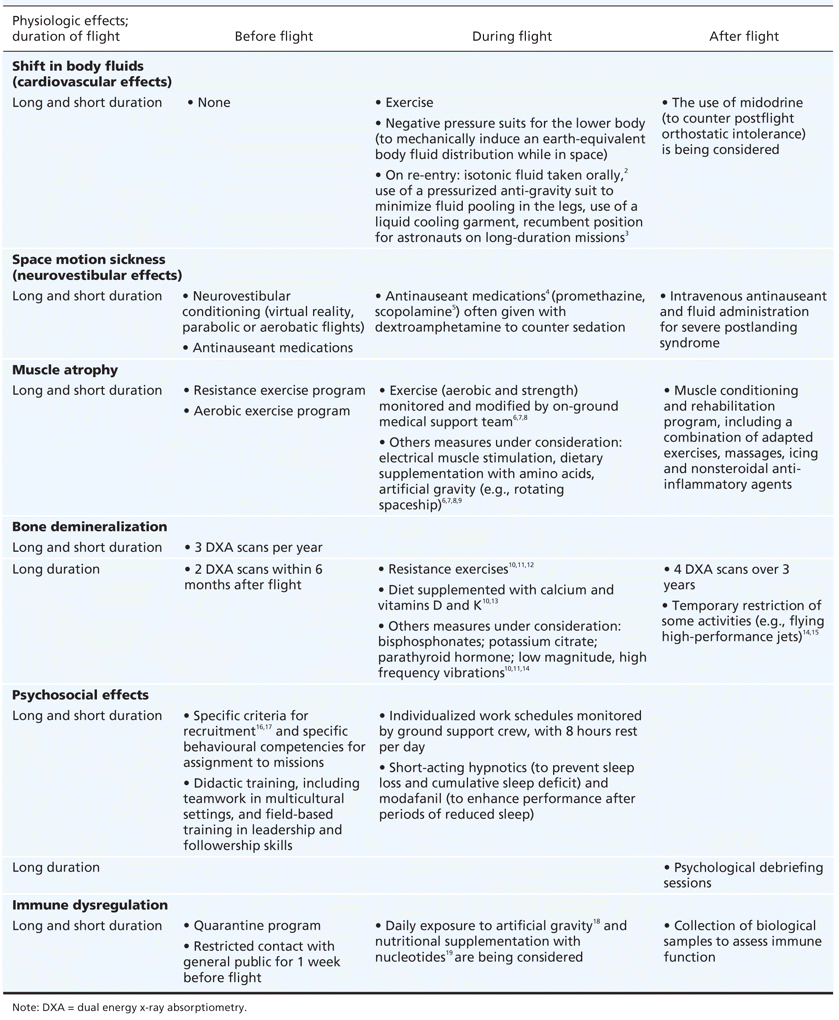
\includegraphics[width=0.95\textwidth]{SJTable4}
	\caption{Countermeasures to minimize risks to astronauts before, during and after spaceflight\cite{Williams2009}}
	\label{acc-counter}
\end{figure}

One strategy for mitigating risks, stressors and ensuring supports for crews in
space is through the development of countermeasures in addition to careful
consideration of crew selection, appropriate training, extreme habitat design,
human factors, social governance supports and societal infrastructures for long
duration spaceflight. (See for instance \autoref{acc-counter}.) Future human
exploration leading to ``staying there'' (\autoref{staying-there}) will need to
design protocols and policies for consent and justice for one-way missions and
strategies for permanent colonisation with ethical micro and meso-social
structures.

Today astronaut crews actively contribute and refine existing technologies and
protocols to ensure best practices and environments for living and working
based on their first-hand experience during space flight or mission; however
the prevalent thought and practice today is essentially terrestrial.
Countermeasures by their very nature, seek to provide supports consistent with
the human need on Earth and thus have an inherent pedestrian and
gravity-centric logic. Mitigating the optical disturbance of zero-gravity for
instance by creating a false orientation with `Up' signs and consistently
angled writing provides crews with short-term adaptation solutions. The need
for Lunar, Martian and general Astro-centric specific counter-measures and
harness-measures will be required in the future if we are to ensure optimum
performance and evolve as an adaptive and empowered space-faring and future
space-dwelling species.


\begin{comment}
Send to BibTeX:
"Acclimation during space flight: effects on human physiology",
David Williams, MDCM MSc, Andre Kuipers, MD, Chiaki Mukai, MD PhD andRobert
Thirsk, MDCM SM. CMAJ • June 23, 2009; 180 (13). First published June 9, 2009;
doi:10.1503/cmaj.090628  © 2009 Canadian Medical Association  www.cmaj.ca
\end{comment}
 
\subsubsection*{Psychological wellness}

The psychological and related physical impacts of long duration space flight
and extended human exploration into space on human performance, social
interactions, group and community interactions, space-Earth relationships and
crew-specific behaviours are critical to operations and overall mission
success. Further research on the sources and impact of long duration space
flight on crew health and incremental risk identification is needed in order to
reclassify behavioural health risks and thus best-plan for eventual human
colonisation of space. The need for autonomous medical care, self-care, remote
care and communications strategies should be considered essential design
requirements for Human Factors and Extreme Design architecture, Crew selection,
pre-flight training, In-flight Procedure, and space-protocols.  

\subsection{Robotic Exploration}
%(to be written by Jan)

By default, much of space exploration today is highly dependent on robotic
systems as well as on support by means of artificial intelligence. From the
early days of space exploration on, humans sent robotic devices and satellites
into space to sense, image and explore the space frontier. However, much of the
robotic exploration systems provide only crude degrees of ``intelligence.''
More often than not, systems in space lag 15 years or more behind technology
available on earth, which is mostly due to safety requirements as well as
extensive research and development cycles within the space industry.  

Another phenomenon which goes along with this is a fundamental dispute over
human vs. robotic space exploration of space. The underlying logic states that
robots will facilitate the groundwork of exploration for humans to follow. At
this stage, the human dream to explore and possibly colonize space is normally
dominated by the premise to move our life support systems into space and onto
other planets.

However, non-augmented human bodies need an earthlike environment almost to
exact earth specifications. Earthlike atmospheres, which are changed by the
very metabolism of the body being in it, water and hundreds of other needs from
complex nutrients, molecules, to exercise, social and spatial requirements.
Ironically, the body that gives us the primary medium for experiencing our
surroundings is also the single largest barrier to traveling and experiencing
space. 

A long-term plan to visit space in human bodies is basically committing to the
idea of bottling up earth and exploring space inside of an ``earth-bottle,''
which entirely separates us from the extraordinary experiences the
interplanetary universe offers us. 

We argue that a new conceptual model to evolve space exploration should be
based on the development of a new kind of humanoid robotics, super-human
artificial intelligence as well as virtual representation of space exploration.
In addition, the development of an inter/intrastellar smart network to connect
all information-based agents, robots, vehicles, nodes and life-support systems
is suggested to provide a collective intelligence approach within space.

Humanoid robots---robots with human-like bodies such as Asimo or
Robonaut---will quickly increase in their sensory capacity, eventually
exceeding perception capabilities of the human body. In limited ways we already
see today how robots equipped with night vision capability, thermal imaging
capability, radar, seismographs, EMI receivers, and so forth augment human
sensing. However, we suggest that such humanoid robots are only the very
beginning of this ``body'' evolution. As described later, exponential advances
in neuroscience, nanotechnology and synthetic biology will allow for a
super-human kind of robots, with many human-like characteristics. However, such
robots can be augmented with sensing and actuation capabilities beyond human
limitations and can be specifically customized for conditions in space. In
addition, the development of a specific ``super-human intelligence'' for such
robots provides significantly higher information processing, problem solving
capabilities, as well as communication characteristics with other intelligences
such as robots, networks, satellites and humans by means of a space-wide
operating system (e.g. ETIR idea ``Intelligent Space Operating System''). Human
intellect can then be uploaded remotely, augmented by means of enhanced
perception/sensing, and experienced individually as well as collectively. Super
Human Intelligent robots for space exploration provide the benefit to be
resistant to adverse conditions within space such as extreme temperatures,
radiation and toxins. By default, they don't require oxygen, food, sleep, or
sunlight and can be designed to be of higher emotional/psychological robustness
compared to humans. Psychological, social and bodily characteristics can be
dynamically shaped to be optimal for individual space missions and can be
adapted over time.  This new kind of robotic super-human space exploration is
meant to open up channels of exploration and experience with a currently
unimaginable level of perceptive richness and extended realism by means of
augmented sensing.  In addition, new kinds of virtual environments,
brain-machine interfaces and multimodal feedback systems will allow us to
navigate such experience at in virtual fashion at increasingly higher
resolution and vividness. This can be shared by everyone on earth rather than
by a few astronauts.  We believe the future of mankind in space can, and will
be more interesting, exciting, and inspiring than the current vision of
exploration with a human earth-bound body -- both can and should happen in a
parallel initially. We believe we can explore the planets not just from the
confines of a space suit or tin can on the surface, but from a spectrum of
physical embodiments, beginning decades ago with space robots that sent back
images for us to experience.  We will then know exactly on earth what it feels
like to stick a feet in the sand of Mars, to go for a space-walk, or to observe
our planet as a swarm of satellites.

\begin{comment}
1. Ellery a. Humans versus robots for space exploration and development. Space Policy. 2003;19(2):87-91. Available at: http://linkinghub.elsevier.com/retrieve/pii/S0265964603000146.

2. Crawford I. The scientific case for human space exploration. Space Policy. 2001;17(3):155-159. Available at: http://linkinghub.elsevier.com/retrieve/pii/S0265964601000200.

3. Fisackerly R, Reimers C, Pradier A. Exploration system technology aspects in the exploration programme of the European Space Agency. Acta Astronautica. 2006;59(1-5):3-12. Available at: http://linkinghub.elsevier.com/retrieve/pii/S0094576506001196.

4. Peter N, Stoffl K. Global space exploration 2025: Europe's perspectives for partnerships. Space Policy. 2009;25(1):29-36. Available at: http://linkinghub.elsevier.com/retrieve/pii/S0265964608001033.

5. 1. Messina P, Vennemann D. The European space exploration programme: Current status of ESA's plans for Moon and Mars exploration. Acta Astronautica. 2005;57(2-8):156-160. Available at: http://linkinghub.elsevier.com/retrieve/pii/S0094576505001116.

6. Horneck G, Coradini A, Haerendel G, et al. Towards a European vision for space exploration: Recommendations of the Space Advisory Group of the European Commission. Space Policy. 2010;26(2):109-112. Available at: http://linkinghub.elsevier.com/retrieve/pii/S0265964610000238.
\end{comment}


\subsection{Space Resources}
%(to be written by Mike)
Human resource consumption increases as the population of the Earth
increases and as each member of the population uses more resources,
but the amount of resources available on the Earth remains fixed.
Fortunately, we as a species are not limited to gathering these resources
terrestrially. While we are facing a shortage of both raw materials\cite{gordon}
and energy\cite{Seboldt2004} here on the planet, both of these resrouces are bountiful
in our solar system and beyond.

This observation is by no means novel. Right now, though, at the dawn
of this new decade, we find ourselves sitting on the brink of an inflection
point with respect to the harvesting of space-based resources and
bringing them back to Earth. For the first time, as a result of the
convergence of several pivotal and game-changing exponentially accelerating
technologies, it will not only be economically viable to supply and
power Earth from space, it will be a necessity.

\subsubsection*{Terrestrial Shortage of Valuable Materials}

There are currently not enough raw materials present on planet Earth
for the world's current population to live with the quality of life
of the modern developed world\cite{gordon}. This shortage clearly
poses a large problem for the sustained growth of humanity in the
upcoming decades, for not only is it desirable for every human being
to have access to the same level of technology as those living in
the developed world, but those in the developed world strive to advance
their technological. Among others, some of the most important of these
scarce materials are platinum group metals\cite{gerlach}.

As these scarce materials are mined and extracted from the Earth,
they become more and more scarce, and as they become more scarce the
cost of mining them and extracting them increases. Fortunately, virtually
all of these terrestrially scarce materials are available in space
and can be found in near-earth asteroids. In the past, the cost of
mining these asteroids and returning their materials to the earth
has been prohibitively expensive. However, in the upcoming five to
twenty years, the convergence of a number of exponentially accelerating
technologies will result in the cost of mining these asteroids decreasing
exponentially. With the cost of mining these materials from the earth
increasing with every passing year, and the cost of mining them from
space decreasing every year, there will be a point in the near future
where it is not only economically viable but economically imperative
to mine asteroids and return their contents to Earth\cite{gerlach}.

There are many advantages of mining near-earth objects for resources
over obtaining the resources from Earth, even aside from terrestrial
shortage. First of all, it is likely that a high percentage prospecting
missions will successfuly find highly valuable asteroids, due to already
well-established science for analyzing the composition of asteroidal
bodies from Earth. The high-grade ore found in asteroids will make
processing (extractive metallurgy) quite easy. No negotiations will
be needed with existing landowners. Additionally, there are no environmental
laws to be dealt with, and mining and waste disposal will not have
any potentially destructive effecst on the terrestrial ecosystem.
Asteroid mining systems will be highly scalable, flexible, and reusable\cite{sonter}.

Additionally, even if there were not a terrestrial shortage of materials
like platinum group metals, there is no doubt that if we had more
of them, it would usher in a new era of abundance on our planet. Imagine
the advances in technology and quality of life that could be made
if engineers could always use the ideal material for the job without
having to worry about price or availability.

Finally, the successful mining of asteroids will be essential to the
ultimate expansion of our species into the solar system and beyond.
Launching heavy objects from the ground in to space makes much less
sense than constructing those objects in space from available resources.
These resources are all available in near-Earth bodies.

Thus, the value of mining asteroids for resources is clear. There
are a number of sub-problems that must be solved in order to successfully
accomplish such a mission\cite{gerlach}. Each of these problems can
be solved elegantly with a combination of exponentially advancing
technologies.

\begin{description}
\item[Remotely mining asteroids without the need for humans. ]Advances
in AI and robotics will make this task cheaper and more efficient,
and cheaper as robotics and microprocessors become cheaper.
\item[Data Collection. ]Improved microprocessors, storage technology,
and sensors will drop the price and enable more and better data to
be collected. 
\item[Mass and performance of spacecraft.] New materials such as carbon
nanofibers and advanced composites will enable lighter structures
to be as strong or stronger than steel.
\item[Launch and Propulsion. ]Advances in launch (particularly beam-powered
launch), solar technology, and energy storage will greatly increase
the efficiency while decreasing the cost, dramatically cutting the
costs of an asteroid mining mission.
\item[Design.] Advances in software modeling and design will dramatically
increase the chance of success and decrease the cost of each mission.
\item[Miniaturization. ]The smaller a mining vehicle is, the more
can be launched per payload and the more fault-tolerant the entire
overall mission can be. Many technologies are getting smaller every
year, and this will dramatically affect the industry.
\end{description}

In sum, it is absolutely essential for humans to mine asteroids for
materials, since Earth is running out of resources, it will be essential
for building space-exploration machinery in place, it will usher in
a new era of abundance on Earth, and the cost of mining space-based
materials will soon be cheaper than mining those same materials terrestrially.
By leveraging a key set of exponentially advancing technologies, it
will for the first time be possible very shortly to mine asteroids
effectively, efficiently, and profitably.

\subsubsection*{Space Based Solar Power}
%(written by Jason) NOTE- I will email Carlos and Davidad the reference material.

An underlying motive for all of human expansion has been the quest for energy.
To early humans this meant the search for food, as food was the only form of
energy they could take advantage of. Later on, our species created ways to
harness other forms of energy through mechanical means---water power, wind
power, coal, oil, uranium. These steady developments led to the expansion of
the human race across the oceans to settle on nearly every habitual space on
Earth.

Today, with a global power consumption of 12TW\cite{Seboldt2004}, we are
reaching the end of the energy supplies we have come to use so commonly. It is
expected that by the year 2020, the global power consumption will be nearly
20TW. It is becoming more expensive and more risky to search for fossil fuels
to power our cities, and the combustion of these fuels is becoming highly
damaging to the environment. Over 85\% of the power used today comes from
fossil fuels\cite{Seboldt2004}. It is generally accepted that the time has come
to focus on powering our world from completely renewable resources, and there
are many resources that can be harnessed; tidal currents, wind, geothermal, and
of course solar. Solar power is unquestionably the ultimate solution to our
energy demands. In fact we have always relied on solar energy, we are just
prefer to use it in it's stored form of a battery called fossil fuels.

When we begin to explore the possibility of harvesting energy in space, rather
than terrestrially, we will create a world of energy beyond what we can imagine
today. The amount of energy in space is far greater than that needed to sustain
the population of the planet for decades to come. For instance, the kinetic
energy in the solar wind is $10^{14}$ MW, or over a million times the current
global power consumption. Collecting solar energy and transporting it to Earth
will not only solve the energy problem, taking everyone out of the ``dark age,''
but will also open the space frontier economically. As soon as the break-even
point is passed, a viable business case for space energy production will
swiftly drive down the costs of launch, as more and more capital comes in from
the energy sector.

\begin{comment}
References:
(NSSO 2007) Space Based Solar Power as  and Opportunity for Strategic Security, 2007
(Chaudhary 2010) Chaudhary, K., Vishvakarma, B.R. Feasibility study of LEO, GEO and Molniya orbit based satellite solar power station for some identified sites in India. J. Adv. Space Res. (2010)
(Seboldt 2004) Space- and Earth-based solar power for the growing energy needs of future generations
\end{comment}

\subsection{Space Science}
%(to be written by Diva)
\begin{center}
\em ``Somewhere, something incredible is waiting to be known''
\end{center}
\attrib{\textbf{-- Carl Sagan\index{Sagan, Carl}}}

Before the 19th century, when the term ``scientist'' was first coined, people
investigating Nature called themselves ``Natural Philosophers'' because they
observed the workings of Nature and tried to extrapolate universal rules that
would enable them to understand the surrounding World. What is the unit of
life? What is the unit of matter? Is the Earth flat? These questions put
forward by natural phylosophers, found an answer as technology started making
its first steps into the era of modern science, thus empowering mankind to look
deep into the structure of matter and far out beyond the atmosphere. As
technology kept progressing exponentially, it allowed scientists to wander into
new and unexplored territories. New questions thus arose: does life exist on
other planets? Can intelligent life be found beyond our Solar System? Can there
be different forms of intelligence? How did the Universe form? How did
humankind evolve from prokaryotes? New fields---astrobiology, exobiology,
planetary science, space-based astronomy---were born to answer these questions,
while existing ones---biotechnology, medicine, neuroscience, synthetic biology%
---started just now extending their reach into outer space. Altogether, these
disciplines fall under the umbrella of a new scientific era, that of Space
Science.  

The comparatively nascent field of Space Science is at the cusp of major
growth, given the technologies available in the next decade. The same curiosity
that has driven technology advancement and continuity over the past centuries
on Earth, has lead scientists just beyond the atmosphere over the past decades
and will, in the comparatively near future, bring humanity to explore and
colonize outer space. Space Science will provide a parallel or a whole new
domain of possibilities beyond our imaginations today. Importantly, it will
bring about new paradigms for the Science that is done on Earth, out of the box
thinking that could feed back into the living system with the potential of
tackling many of the still unsolved or unsolvable problems. These underlying
features inevitably set apart Space science from the rest of the modern
sciences. One could say that today is the beginning of a new era in Science, an
era in its own right, which will see its climax in the human colonization of
other Earth-like planets and the exploration of other solar systems. 

\subsection{Space Education/Evangelism}
%(written by Jason, edited by davidad)

A key underlying problem to the limit  of humanity's progress in space is that the majority of the human  species is uninterested in space. Activities in space today do not  inspire the awe that they once did: instead of watching astronauts walk  upon the surface of a celestial body for the first time, today, if we're  lucky, we get to watch them repair the toilet on the International  Space Station. Educational outreach is a good start, but we need to  connect humanity to space in a more natural way. Global warming is now  perceived as a threat so compelling that most people believe we need to  do something about it. But this threat is dwarfed by that of remaining  on this planet indefinitely.

NASA's  education program attempts to make space and the STEM (Science  Technology Engineering and Math) curriculum exciting for students, but  they do it without an understanding of the progress exponential  technologies will have on the space industry. Students today rarely  realize that when they grow older they will have a completely different  tool set with which to tackle space. We should teach them what the world  will be like in a decade or two and excite them on the possibilities  they can create.

In  all instances of educating the public on the importance of space, from  youth to the elderly, opening the space frontier is never presented as  an explicit need---which it is. Space is often considered to be  primarily beneficial as an engine for creating technological spin-offs,  but even if space exploration paid no technological dividends, it would  still be crucially important. People don't appreciate the voyage of  Christopher Columbus to the Americas primarily because of the new  sextant developed for the journey that was eventually spun off to the  private sector and used in merchant shipping.

It is human nature that we need to ``see it to believe it,'' and maybe this is what is holding back humanity  from understanding why space exploration is a necessity for survival.  Until ordinary people can experience space through their own eyes, the  possibilities that it holds will not be fully understood. What will  happen when the first child can see our home from space, or when the  first ballet dancer experiences weightlessness, or when a paraplegic is  given mobility again? Let's not just tell humanity about space, let's  give them access to space.


\subsection{Insuring Humanity}
%(to be  written by davidad)


\section{Exponential Technology Areas}
% Summary list\ldotsof what you considered, based on the SU tracks, for example

In this report, we will illustrate a number of opportunities to address the
above problems with exponential technologies. This section serves as a brief
overview to each of the exponential technology areas.

\subsection{AI and Robotics}

% [Can we make this paragraph a vision statement rather than a historical statement?
% Something more from http://su-etherpad.com/tpspace-The-Real-New-Space ?]
%   [davidad: this is intended to be a historical orientation, but feel free to add a
%    third paragraph that is more visionary in tone.]

In the broadest sense, the fields of AI and robotics strive to make non-human systems able to perform human tasks%
%Is this too limiting a view of AI and robotics? -- Will they just be worker tools, or the
%beginnings of a future of extraordinary intelligence and physical capabilities?)
, or other difficult tasks that are helpful to humans. Robotics focuses on the necessary physical capabilities, while AI focuses on the necessary mental capabilities. At present, AI systems are capable of solving a plethora of individual problems, each of them far more swiftly and accurately than a human could; but no robot is capable of loading a dishwasher yet.
% I would not make this point, as Robots already wash our dishes today far better than
% humans do (including total disinfection), and don't do it at all the way we do (contained
% machines). Planes also don't fly like birds, but we might say they are far better for our
% purposes.
This phenomenon is represented by the term ``narrow AI'': each AI system today is typically helpless outside the situation it was designed for. These systems solve problems such as searching the Internet, routing FedEx packages, military logistics, or playing chess. However, it has been predicted that in the future, we wil develop what is known as ``strong AI'': an AI system that nears human levels of tolerating uncertainty, and can generate original solutions to problems hitherto unseen and unanticipated by the designers of the AI.

\subsection{Biotechnology}

We currently live in the Renaissance era of Biology. Molecular biology along
with computer science is the fastest growing science of the past four decades.
This rapid development is due to a consecutive line of major milestones that
include: Solving structure of the DNA, Deciphering the genetic code, Genetic
engineering via restriction enzymes, The PCR machine, Microarry technology, The
completion of the human genome project, microfluidics technology and more. The
vast array of tools and knowledge gave rise to a growing branching of
sub-fields of Molecular Biology that include Genetic engineering, Biophysics,
Protein design, Protein fold prediction, Bioinformatics, Computational biology,
Systems Biology and most recently, Synthetic Biology.
 
In the following paragraphs we shall outline the most notable exponentially
growing molecular biology fields and methods:
 
Genomics is the extension of genetics to the scope of full organisms' genomes.
Genomics is rapidly developing in the reading capabilities of DNA which is
regarded as ``DNA Sequencing,'' the artificial generation of DNA polymers which
is regarded as ``DNA synthesis'' and the comprehension of the genetic
information.
 
DNA Sequencing capability is exponentially improving ever since the human
genome project was launched. The first significant technological leap is owed
to the contribution of Dr. Craig Venters that introduced the ``Shotgun'' method
through his company Celera. An active and highly innovative industry competes
by introducing diverse technologies for sequencing which may be very different
in method. Although there still is no one technological golden standard, the
speed of sequencing and amount of DNA material that can be processed in
parallel is exponentially growing whereas the price is rapidly dropping. This
could be exemplified by the amount of DNA sequences submitted to Genbank, a NIH
funded DNA repository (see figure).

The vast amount of genetically available material paved the way for the
Bioinformatics fields that was essential for the assembly, interpretation and
pattern recognition of the accumulated data. Bioinformatics in turn grow
rapidly and branched into several sub fields that specializes in genes (``coding
regions''), regulatory elements (``intergenic regions''), gene expression
analysis, systems biology and computational biology. Systems biology that aims
to achieve the co-functioning comprehension of a large set of genes and
proteins is rapidly growing as can be seen by the amount of grant funds the
field receives (see figure).
 
Upon the completion of the human genome project in 2000 by both by the
international consortium and the Celera private venture the tipping point and
rise of the post-genomic era began. The draft to our genetic software was
accessible to study for the first time in human history, and genes where being
studied in large sets of thousands rather than one at a time.  A similar era is
about to embark soon, as full genome sequencing prices will fall sufficiently
to enable a multi-genome era where humanity will hold a large set a genomes by
different individuals, enabling comparative genomics, the exhaustive comparison
of entire genomes.
 
DNA synthesis capability, albeit lagging behind the DNA sequencing technology,
is also advancing by a verity of methods, and synthetic DNA grows longer and
cheaper rapidly. As in the DNA sequencing arena, Dr. Craig Venters contributed
greatly to this field to and currently holds the record for the largest
sequences of artificially generated DNA.  Long synthesized DNA is driving the
emerging field of synthetic biology that aims to fabricate novel life forms.
The current state of the art is a partial generation of a bacterial organism.
 
Proteomics is the extension of Biochemistry to the scope of full organisms'
proteins.  Proteomics is rapidly developing in the reading capabilities to
solve the 3D structure of proteins by means of X-ray crystallization and NMR
studies as can be seen by the exponentially accumulation of protein structures
in PDB, the protein data bank (see figure). Although the 3D structure of most
proteins is known to be directed by the amino acid sequence of the proteins,
the question of inferring the structure from the sequence which is also known
as ``the protein folding problem'' is still largely unsolved and is on of
Biology's holy grails. However, the computational prediction of the structures
are growing increasingly better due to superior heuristics, vast amount of
biological raw data and extended computation capabilities, and it is widely
believed this challenge will be eventually solved. The ability to comprehend
the correlation of protein structure and function will enable the rational
protein design and will open a virtually limitless space of synthetic proteins
with properties that to date do not exist in nature. A mature protein design
field could correct for most genetic defects along with the transplantation of
genes via Gene therapy methods, create new genes and produce new bio materials
and biological drugs such as hormones and antibodies. To date, protein design
is limited to semi-random in vitro evolution methods, partially driven by
rational thought and by chimerical approaches of modular construction of
proteins based on naturally existing scaffolds.
 
The microarray technology and its subset DNA-chips is yet another disruptive
trend in biology that enables a vast readout of all the expressed genes within
a cell by assessing the presence of mRNA transcripts. This technology, along
with the exponential advances in DNA sequencing, greatly contributed to the
generation of the Bioinformatics field, and to its sub branches, gene
expression regulation and Systems biology. The microarrays that were at first
extremely expensive, unreliable and with a relatively small number of
biomarkers, are now commonly used, as can be seen in the elevated number of
publications that address microarray data, and they are rapidly growing
cheaper, larger and robust. To date there is still no gold standard to the
optimal mathematical correction algorithm for their analysis, and the field of
microarray analysis quite active.
 
Another disruptive and rather new technology is Microfluidics that enables
micro manipulation and experimentation on single cells via liquidous apparatus
with miniature compartments. Microfluidics enables experimentations that have
previously not been feasible.
 
In the near future, we will be readily reading, generating, transplanting,
manipulating and creating genetic and protein material, capability that will
enable us to reshape life forms including humans.
 

\subsection{Nanotechnology and Materials Science}

The first tools that humans used were simple sticks and stones, native ``bulk''
materials from the environment. Certain rocks were chosen for their hardness,
or for their sharpness when cleaved, while certain sticks were used for their
light weight and as tools requiring aspect ratios that are unattainable using
rocks. Later these bulk materials were combined into things that enabled
functions that were more than the sum of the parts, such as stone axes, animal
traps, and wheeled vehicles.

In a similar way, we are barely beginning our technological evolution in space
and are using many bulk materials, for example the planned Mars Curiosity rover
is made mostly of aluminum and uses two-dimensional monolithic computation
elements. The next step, and the goal of nanotechnology and materials science,
is to discover the structural, electronic, thermal, and other physical
properties of nanoscale materials and learn to harness these properties to
create new or improved functionality, both structurally and on the scale of
sensing and computation elements. These properties that may be inferior in bulk
materials or perhaps not even exist on the macro-scale.

\begin{comment}
Nanostructured materials and nanoscale devices will be precisely engineered on
the molecular scale to harness these properties.  Structurally, they may be
stronger, lighter, or more flexible, such as carbon fiber. They may promise
improvements on existing technology, such as graphene as a replacement for
transistors, or heretofore unforseen devices, such as graphene as an atomically
thin vibrating two-dimensional membrane for mass sensing (while other
materials, even thin materials are three-dimensional). In addition, since
biological organisms are a vast assemblage of nanomachines, the line between
artificial nanoengineering and nature may be blurred in many applications.
\end{comment}

The enabling factors for continued improvement and innovation at the nanoscale
reside in both funding new research and in an applications-centered,
business-driven approach. They may reside in a shift from old ways of thinking
and an agility to absorb new technologies as they become available.

\subsection{Information Technology and Networking}

The exponential nature of Information Technologies and Networking is a well
established phenomenon. In 1965, Intel's co-founder Gordon Moore noted that the
number of components in integrated circuits had been doubling roughly every two
years since their invention in 1958, and predicted that the doubling trend
would continue for at least another decade. Since then, and more than forty
years later, Moore's ``law'' continues to signal the evolution of processing
speed, memory capacity, hard- disk storage, power consuption, transistor cost,
and many other applicable metrics that seem to lay, roughly, on exponentially
increasing (or decreasing) curves. (See \autoref{moores-law}.)

\begin{figure}
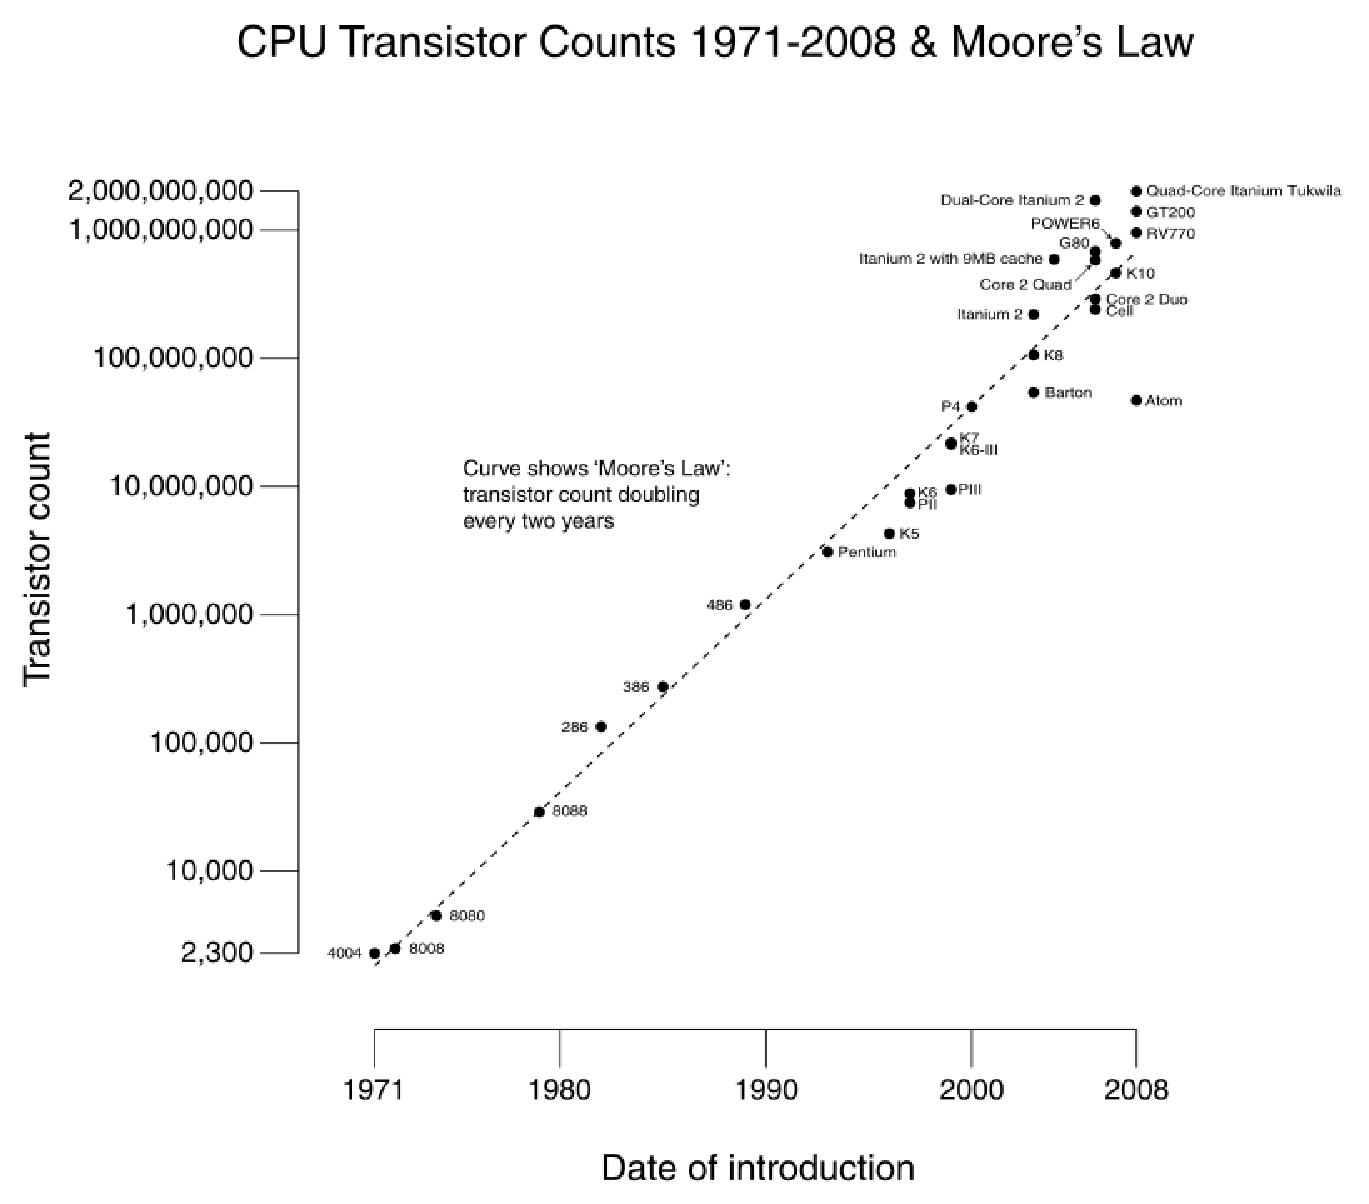
\includegraphics[width=\textwidth]{Transistor_Count_and_Moore's_Law_-_2008}
\caption{Transistor count and Moore's Law}
\label{moores-law}
\end{figure}

It is remarkable that these exponential trends have survived many technology
changes, and some technological paradigm shifts, without ralenting even through
global crisis or other political and economical turmoils. An industry-wide
belief in the nature of these exponentials has led companies to invest billions
of dollars in the process of finding the next doubling factor before the
competition, and drove many to describe Moore's law as  the ``self-fulfilling
prophecy'' of the electronics industry. However, and even though every few
years new technical bottlenecks seem to suggest that Moore's Law might be
getting to an end, our current understanding of the fundamental limits of
computation shows that there is no fundamental reason why computational density
should not keep increasing at its exponential pace for the forseeable future.

Over the last five decades, the exponential evolution of electronics has
played a fundamental role in many of the scientific and technological
achievements of humanity, and has been a fundamental enabler of global trade,
the increased efficiency of value chains and the onset of what is called the
knowledge economy. The Internet itself, still in its infancy, has
revolutionized the way we do business, collaborate and interact with each
other, and the same technology, in the hands of billions through mobile phones
and its descendants, is predicted to play a fundamental role in integrating the
next four billion people in the base of the pyramid to the global economy and
to a global society. The astronomical increase in our capacity to generate,
store and process information is leading fundamental changes in the way we
think about and do science. Many other scientific disciplines, including, most
notably, biology, are now increasingly becoming information sciences, and the
exponential trends of information technologies spread to these disciplines and
help put them in their own exponential paths. 

We expect these trends to continue and evolve in the short term, and over the
next few decades, to show an increasing paralellization of today's
architectures, increasing interconnectedness, increasing miniaturization, new
human-machine interfaces, new machine-to-machine interfaces, sensor and
actuator networks; embedded computational systems in everyday objects;
distributed, decentralized platforms for data acquisition, storage and
processing; ubiquitous, high-bandwith networks; high-quality augmented/virtual
reality with haptic interfaces; implantable bio-electronics; new computational
paradigms for high-performance, massively parallel computation; new
computational paradigms for energy-efficient and low heat computation.

At the same time, we expect Information Technologies, Computing Systems and
Networks to impregnate, merge-into and drive the convergence of Biotechnology,
Nanotechnology and Neurotechnology, to a new integrated technology realm at the
nano-scale.


\subsection{Neurotechnology and Medicine}

The human beings through research and technology have begun to understand the
nature and mysteries of the Universe. However, Space is a harsh environment,
and technological advancements in material science, robotics, power generation,
and medical equipment will be required to ensure that astronauts survive
interplanetary journeys and settlements. In addition, operational challenges,
such as the management of life-support systems, food and nutrition, medical
care, and psychosocial health due to long-term confinement, will have an impact
on human health during long-term space missions and more even if we think to
settle and to stay on other planets or regions in our Solar System.
 
Since the human is considered to be a critical system of space flight in the
same way the propulsion, thermal, and power are critical systems to space
flight, the searching of opportunities where accelerating technologies could be
possible solutions in these issues in the coming future, is warranted.
 
Why go into space when we have so many problems here on Earth? It is a
legitimate question as unfortunately not enough people have been made aware of
the vast benefits the space program provides that increase the quality of our
daily lives. Applications on Earth of technology needed for space flight have
produced thousands of ``spinoffs'' that contribute to improving several fields
including medicine, biotechnology, and neurosciences\cite{TheSpacePlace2004}.
One small example is the Hubble Space Telescope technology which was used in
the Charge Coupled Device (CCD) chips for digital imaging breast biopsies. The
resulting device images breast tissue more clearly and efficiently than other
existing technologies. The CCD chips are so advanced that they can detect the
minute differences between a malignant or benign tumor without the need for a
surgical biopsy. With over 500,000 women needing biopsies, this technology saves
time and money for this procedure versus surgical biopsy. 
 
At the same time, accelerating technologies in medicine and neuroscience should
help to solve huge problems in human space exploration and ``staying there,''
including better methods and techniques in the basic and clinical research,
which are the basis for new knowledge and the source for new technologies. 
 
Medicine tools that could help solving grand challenges are immersing in
biotechnology, nanomedicine and nanomaterials, robotic, artificial
intelligence, bio-engineering, and bio-informatics. More specifically, the
broad spectrum of sensors and biotech for prevention, and early diagnosis of
the health problems, new materials for radiation protection, autonomous medical
care (AI, robotics, bioinformatics) for diagnosis and treatment, and tissue
engineering for recovery, are some interesting examples where exponential
technologies should be involved.
 
Neuroscience research helps us to describe and understand how the brain
controls behavior. One of the critical tools is the recording equipment which
helps us to study the neural signals during behavior. While noninvasive neural
signal recording techniques, such as electroencephalography (EEG) and
functional magnetic resonance imaging (fMRI), are getting more precise and
easier to operate, their costs are also dropping \cite{mri1991}. As these
equipments are more affordable for the public, more neural recordings from
individuals are available to study a wide range of problems. The exponential
increase in hardware and software tools and the available data help the
development of statistical models for different medical applications, such as
personal health diagnostics.
 
Another trend observed is the decrease in computational time for non-invasive
medical diagnosis through computer tomography (CT), MRI and positron emission
tomography (PET) as the computational power exponentially increases through
techniques like parallelization. Meanwhile, for instance, PET detectors are
getting smaller at an even faster rate, offering higher resolution data
\cite{neuroimage2004}.  \autoref{neuro1} shows that improvements in run time
alone are not sufficient to meet the computing demands for future PET scanners. 

\begin{figure}[htbp]
\centering
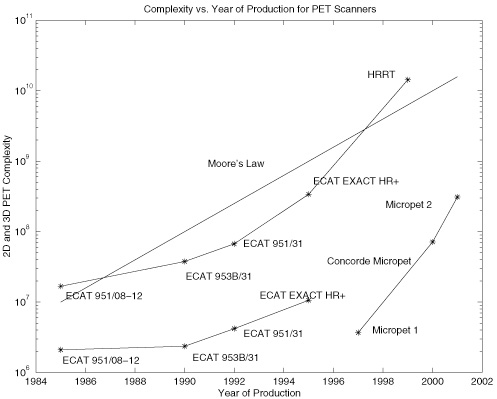
\includegraphics[width=4in]{neuro1.png}
\caption{Illustration of the approximate order of computational complexity for
2D and 3D clinical and small animal scanners shown in comparisons to ``Moore's
law'', the observation that single-processor computing power doubles roughly
every 18 months \cite{neuroimage2004}. The lower curve for the ECAT systems
represents 2D complexity, the upper curve represents 3D complexity.}
\label{neuro1}
\end{figure}
 
Significant improvements can be also found in neural prosthetic devices. Using
implanted electrodes to deliver electrical stimulation to the sensory nervous
system, cochlear implants have been well developed for the deaf to hear and
retinal implants are under FDA trials for the blind to see. \autoref{neuro2}
from \cite{Zeng2004} demonstrated the improvement of sentence recognition of
cochlear-implant users with more recent models. Custom motor prosthetics like
robotic arms with high dexterity are developed for patients who lost their
limbs. Paralyzed patients can now interact with the world with brain computer
interface (BCI). The exponential increase in computational power also allows
researchers to simulate large neuronal network and the resulting knowledge
benefits the development of better neural prosthetic devices.
 
\begin{figure}[hbtp]
\centering
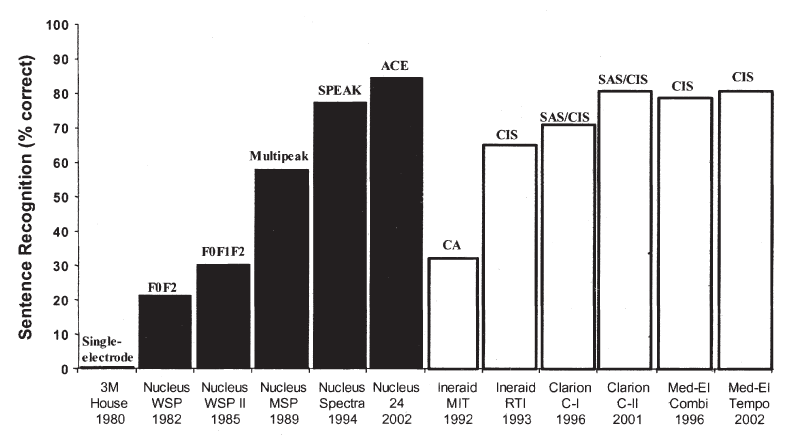
\includegraphics[width=5in]{neuro2.png}

\caption{\justify Sentence recognition of cochlear-implant users \cite{Zeng2004}. The
x-axis labels show the type of device, the processor model, the place where the
study was conducted, and the year the study was published. The y-axis shows
percent correct scores for sentence recognition in quiet. The scores in
cochlear implants developed before 1994 were averaged from investigated studies
published in peer-reviewed journals. The score in devices developed thereafter
were obtained from company-sponsored clinical trials that had also been
published in peer-reviewed journals. Besides ``single-electrode'' for the
3M/House device, the text on top of the bars represent speech processing
strategies including SPEAK (Spectral PEAK extraction), ACE (Advanced
Combination Encoder), CA (Compressed Analog), CIS (Continuous Interleaved
Sampler), and SAS (Simultaneous Analog Stimulation).}
\label{neuro2}
\end{figure}
 
\begin{comment}
REFERENCE
[MRI] http://www.diagnosticimaging.com/display/article/113619/1219412
[PET] http://neuroimage.usc.edu/ResearchPETComput.html
[ZENG] Fan-Gang Zeng, “Trends in Cochlear Implant”, Trends Amplif. 2004;8(1):1-34
\end{comment}


\subsection{Policy, Law, and Ethics}

We are not in a position to fully analyze the far-reaching consequences of
near-term steps by space agencies and private space entrepreneurs, however we
can set about to establish a  context for critical evaluation of our
motivations and hesitations at the Singularity University during the 2010 GSP.
This is a time to develop a culture of intense questioning and reflexivity,
weighing up the pros and cons of social and education value, economic and
political drivers, scientific benefits, risks, the battle for sovereignty
between nation states; time readiness, and the lessons learnt from past human
endeavors at each stage of mission  planning and undertaking. Particular
attention must be paid to our obligations and restrictions, the differences of
moral standing and the agents behind them; the intrinsic and instrumental
values of global peoples and the core truths of our calling, in order to plan
effectively and to garner new insights and knowledge for wider reaching
solutions to terrestrial concerns so that we can leverage exponentially
advancing technologies for the benefit of humanity, the planet and the future
of our activities in space. We have a responsibility to boldly stay to serve
legitimate interests as a peaceful, well-meaning people and the opportunity to
explore new ways of seeing life, and space, from a whole new perspective. 

It is posited that if we are to actually improve standards of living on Earth
through space by  generating economic opportunity; providing access to new
resources (material, intellectual and so on) then we need to bring about the
prospect of rapid technological development, the cross-fertilization of ideas,
new visions and shared dreams for the benefit of all human-kind and this begins
with the power of the questions we ask ourselves, and the declarations we make
for our future generations. 




\section{Exponential Technology Opportunities}

\begin{comment}
\subsection{Classification of opportunities}

We offer a brief taxonomy of the problems that exponential technologies need to
help overcome during the next three decades in order to facilitate the
exploration and colonization of space. For each area in this taxonomy, we
explore the role that each exponential technology might play.

\begin{enumerate}
	\item AI and Robotics \item   Biotechnology \item  Nanotechnology and Material Sciences \item  Information Technology and Networking \item  Neurotechnology and Medicine \item  Policy, Law and Ethics \item Entrepreneurship 
\end{enumerate}

The goal of these definitions is twofold: to map for future reference
our current understanding of the relative role of each of the
exponential technologies and solution domains, and to help us focus our
in-depth analysis of conceptual solutions to those areas that appear
more fruitful.
\end{comment}

$\ldots$For each of the sections below, we discuss the current state of the art,
related exponential technologies, potential benefits, convergences with other
technologies, and potential barriers to adoption.

\secttoc

\subsection{10-year Time Horizon}


\subsubsection{Cheap Spacecraft for Developing Nations}

\begin{description}
\item[Application:] Use cheap spacecraft as a way to enable developing countries to get involved in space.

\item[Problem:] Third world countries are cut off from technology and science in many ways, and often the general public in such countries don't understand what space is and Earth is just a small part of a larger universe.

\item[Opportunity:]
Imagine the headlines: Ethiopia launches their own satellite.If we give developing countries the tools to build and launch their own {\emph useful} satellite at a low-cost (via increasing capabilities of satellites and dramatic reduction in cost), we can:
\begin{enumerate}
\item get 3rd-world countries more involved in space and give them a greater understanding of the world we live in
\item Show the world that space is opening up to all people, and becoming increasingly cheaper to get involved.
\end{enumerate}

\item[Enabling technologies:]
The increase in computational power and decrease in cost is enabling satellites to be built at fractions of the current cost.

\item[Who is doing it:]
\hfill\begin{enumerate}
\item Chris Boshuizen and a team of NASA Ames Research Center engineers launched two Nexus One cellphones to 30,000 feet in July 2010, with plans to launch them to orbit in 2011 \cite{McNally2010}.
\item Bob Twiggs, inventor of the CubeSat, is working on launching eight ``pocket CubeSats'' into orbit in 2011. The cubes are an eighth of the volume of standard CubeSats at roughly 5 centimeters, and are expected to cost less than \$25,000 each with full capabilities \cite{Patel2010}.
\end{enumerate}

\item[Time Scale:] The materials and parts to launch a satellite for less than \$10,000 and eventually \$1,000 is approaching over the next five to ten years \cite{Patel2010}.

\item[Significant Bottlenecks:]
The largest bottleneck isn't the technology. Rather, it's the ability to acquire philanthropic funds for developing countries. Since most countries in Africa don't have the money for clean water or sustainable energy, this idea would have to be sold to philanthropists as a means to educate people in a way that enables them to build their own economy and future space program.
\end{description}

\subsubsection{DIY Spacecraft}

\begin{description}
\item[Application:] Build a satellite architecture that is on the order of hundreds of dollars to launch. Allows for individuals to own and operate their own missions.

\item[Problem:] Creating the business case. Creating the communication system to control and send/receive data from the space crafts.

\item[Opportunity:] With current technology a satellite can be made to sizes within 10 cm on a side and costing the price of a personal computer. With the advancements in nanotechnology, computing, and AI/robotics these spacecrafts will continue to shrink exponentially in size. If we can launch 1000s of these in one rocket the cost per satellite becomes very low.

Each launch will release a swarm of satellites that can serve many purposes. First, because each satellite is identical, all that needs to change to change its mission is the software program, which can be uploaded from ground. This means individuals can own or rent a satellite or any part of the swarm to operate their individual mission, that they create of find through open source software sharing. Monitor global warming from your desktop live, create science fair or research projects, take your own ``pale blue dot'' picture. Google may decide to buy or rent an entire swarm and take Google Earth live giving users incredible benefits such as Instant disaster relief monitoring, The best ideas are the ones that haven't been though of yet.This idea WILL open the space frontier to everyone on Earth.

\item[Estimate of the Potential Benefit:] This technology will be the next best thing to actually putting people in space. It will allow them to see space through their own eyes, which could in turn help motivate the opening of the space frontier.

\item[Who is doing it:] NASA Ames team (Chris Boshuizen, Matthew Reyes, William Marshall), many university Cubesat groups.
\end{description}

\subsubsection{Open Source Cube Satellites}

\begin{description}
\item[Application:] Open source/open cube satellites for development (OSCS)

\item[Problem:] Developing countries more often than not have no direct access to satellites and little
influence on application development, such as remote sensing, communication, and science.

\item[Opportunity:] OSCS can provide a new platform for developing countries to improve data
analytics for development. On open source/open access model is apt to spark innovation in areas
such as remote sensing for pandemics, resource identification, communication, education,
engineering, etc.
%USE of NASA CUBESAT ANNONCEMENT  for 2011 possible.
\cite{cubesatlaunch}

\item[Exponential Technologies:]    Nanotechnology, Computing, and/or
Networks.

\item[Grand Challenges:] Getting There, Space Science

\item[Other Connected Ideas:]   Intelligent Space Operating System (ISOS)

\item[Estimate of the Potential Benefit:]  Significant benefit for developing countries if combined
with terrestrial communication systems. Financing can be achieved through World Bank and
NGO’s with the benefit that loans/donations are transparent (Satellite/infrastructure).

\item[Who is doing it:]
\hfill\begin{enumerate}
\item NASA
\item ESA
\item JAXA
\item MIT
\end{enumerate}

\item[Time Scale:] Immediately, increasingly cheaper in future

\item[Convergence:] Nanotechnology

\item[Significant Bottlenecks:] Cheap Access to Space
\end{description}

\subsubsection{Intelligent Space Operating System}
\label{idea:isos}
\begin{description}
\item[Application:] Intelligent Space Operating System (ISOS)

\item[Problem:] Robotics, AI and communication systems for space more often than not are designed
in isolated fashion. Hence devices and data transmission is mostly non-interoperable, isolated
with great redundancies.

\item[Opportunity:] An Intelligent Space Operating System provides an open ecosystem for AI,
communication systems and satellites, as well as robotics to tie in by means of standardized
APIs. Parts of such ISOS can be open-source and reconfigurable. Open access, open purpose, is
granted as much as possible. AN ISOS ideally encompasses all technology within space and
provides unique identifiers (IPs with encrypted authentication for safety/privacy). Similar to the
earthbound internet (of things) the ISOS provides connectivity, packet switching and
intermittent storage, smart communication processes and optimal routing, satellite access, swarm
satellite tie-in, spacecraft and extraterrestrial station communication, inter and intra-stellar
communications, earthbound internet access and geostationary satellites, real-time as well as time-
buffered information transmission, and inter-robotic communication.

\item[Exponential Technologies:]    Nanotechnology (Microsatellites), Computing Networks, Laser
technology, Solar Panels/energy

\item[Grand Challenges:] Robotic Exploration/ Communication \& Information Networks

\item[Estimate of the Potential Benefit:]  Eradication of redundancies, standardization, smart
information transmission.

\item[Who is doing it:]
\hfill\begin{enumerate}
\item Google
\item NASA
\item ESA
\item JAXA
\end{enumerate}

\item[Time Scale:] Incremental growth during the next years, inclining growth with evolution of microsatellites, exponential growth as soon as cheap access is possible.

\item[Convergence:] Nanotechnology

\item[Significant Bottlenecks:] cheap access to space, but not essential
\end{description}
 
    \subsubsection{Intelligent Environments for Colonization} 
    \label{i2e}
\begin{description}  \item[Application:] -
 
   \item[Problem:] Extraterrestrial habitats for human space exploration  must provide a high level of sensing capabilities to assure life  support. If humans are out to colonize space, long term needs for human,  animal and plant survival must be met.
  
   \item[Opportunity:] Smart environments are already emerging on earth.  Due to innovation in sensor networks, sensor sophistication and  miniaturization, an increasing amount of environmental conditions can be  assessed. Sophisticated data analysis techniques allow for better  modeling of conditions and actions to be undertaken. Smart environments  such as a planetary or orbital station can connect to other nodes within  the Intelligent Space Operating Systems (see \autoref{idea:isos}) for optimization of  the overall space system state.
 
   \item[Exponential Technologies:] Nanotechnology, Biotechnology,  Computing, Networks.
 
   \item[Grand Challenges:] Habitats, biospheres, networks and  communication.
 
   \item[Other Connected Ideas:]  ISOS (Intelligent Space Operating  Systems)
 
   \item[Estimate of the Potential Benefit:] Essential for survival and  colonization, interconnectivity with other habitation nodes allows for  overall system optimization.
 
   \item[Who is doing it:]
  \hfill\begin{enumerate} 
     \item NASA
     \item Living-Planit
     \item Smart cities  MIT
    \item Responsive environments group MIT
     \end{enumerate}
 
   \item[Time Scale:] 5-10 years.
 
   \item[Convergence:] Nanotechnology and exponential ICT. Sensor development  and miniaturization.
   \end{description}

\subsubsection{Microbial Fuel Cells}
\label{microbe-fuel}
\begin{description}
\item[Application:] The use of  microbial fuel cells to generate power within
the Life Support Systems and any  different energetic applications in
spaceflight  or planetary stations could be a suitable, renewable and
efficient way of produce removable  energy.
\item[Problem:] The energy use for  life support systems and other
applications  during spaceflight and space station are restricted to
functions previously planned. The use  of additional energy system
could help  in building successful new life support systems and closed
loop systems.
\item[Opportunity:] \glspl{MFC} are devices  that use bacteria as the catalysts to
oxidize  organic and inorganic matter and generate current \cite{Rao1976}
. Electrons produced by the  bacteria from these substrates are
transferred  to the anode (negative terminal) and flow to the cathode
(positive terminal) linked by a  conductive material containing a
resistor,  or operated under a load (i.e., producing electricity that
runs a device). The construction and  analysis of \glspl{MFC} requires
knowledge  of different scientific and engineering fields, ranging from
microbiology and electrochemistry to  materials and environmental
engineering.  For example, was observed that when a water-soluble
distyrylstilbene oligoelectrolyte  (DSSN+) was added into bioreactors,
these  molecules were preferentially accumulate within cell membranes
and were used as the electron  transport mediator increasing the \glspl{MFC}
performance \cite{Garner2010}. In addition, Yuan et al. reported a novel bioelectrochemical  system to effectively reduce organic pollutant with utilization of the energy derived from a
microbial fuel cell \cite{Yuan2010}. In such a system,  there is a synergetic effect
between the  electrochemical and photocatalytic oxidation processes.
Both systems show great potential to  produce energy and to be part of
a closed  loop system for space exploration.
\item[Exponential  Technologies:] Biotechnology, Synthetic biology.
\item[Grand Challenges:] Human  exploration (staying there, life support systems)
\item[Other Connected Ideas:] Closed  loop systems, bioconductors
\item[Estimate  of the Potential Benefit:] A better source of energy which can
be used in space propulsion and  activation of improved life support
systems.
\item[Who is doing it:] \hfill
\begin{enumerate}
\item Dr. Bruce E. Logan Hydrogen  Energy Center, 212 Sackett Building,
Penn State  University, University Park, Pennsylvania
\item Dr. Shi-Jie Yuan, Department of  Chemistry, University of Science \&
Technology of China, Hefei, 230026,  China
\item Dr. Korneel Rabaey, and Dr.  Jeffrey M. Foley, Advanced Water
Management  Centre, Gehrmann Building, The University of Queensland,
Brisbane, Queensland 4072, Australia
\end{enumerate}
\item[Time Scale:] 5 years
\item[Convergence:] Being in the area  of bioreactors, this technology could
benefit big  challenges in up-cycle and energy areas.
\item[Significant Bottlenecks:]  \gls{MFC} research is a
rapidly evolving field that lacks  established terminology and methods
for the  analysis of system performance. This makes it difficult for
researchers to compare devices on an  equivalent basis.
The most of \glspl{MFC} require large volumes to produce more energy which is
a problem in launch costs.
\end{description}

 
\subsubsection{Polyethelyne/Biopolymer Radiation Shield} 
\label{biopolymer}
\begin{description}  \item[Application:] Generation of hydrogen rich polymers to shield the  inside of shuttles/inflatable inhabitable units from ionizing particle  and high energy electromagnetic radiation
\item[Problem:] 
The Earth’s magnetosphere prevents  protons, electrons and heavier nuclei that are continuously ejected by  the Sun from reaching the soil. Also, Earth's atmosphere blocks some of  the visible and infrared electromagnetic radiation, almost all the  ultraviolet and all the X and gamma rays. While humans have evolved a  system of UV protection involving melanin, no shielding is naturally  provided from particle radiation.

Human  exploration and colonization, as well as orbiting astronauts and  satellites in the shorter term, will greatly depend on the advances in  radiation protection technology, since the planets/moons/asteroids that  we will be in reach of most probably will not have an inherent  magnetosphere that will protect us.

Especially dangerous are the flares and coronal mass ejections generated by the  Sun in an observed nonstationary Poisson process, i.e. random  distribution \cite{Aschwanden2010}. These particles have  sufficient energy to get through any shielding material currently used  in space shuttles/space suits as well as the Earth's magnetosphere and because they are  unpredictable they constitute a major threat. \cite{solarsystemexplore}

Importantly,  the use of improper shielding material might cause the generation of  secondary radiation, i.e. acceleration of a charged particle through  deflection of another charged particle, which increases the probability  of absorption from the organism \cite{NCRP}.
It is therefore vital that  complete ionizing radiation protection be established before any human  colonization missions. 
 
\item[Opportunity:] It has been  observed that shielding materials of low atomic number, such as  hydrogen, are more effective against cosmic radiation (high energy  particle radiation from outer space) than, say, aluminum, because they  reduce the production of secondary radiation particles \cite{Aschwanden2010}. This can be extended to other ionizing high energy  particle radiation brought by the Sun. Polyethylene, because of its  hydrogenous nature, has been extensively used for shielding of crew  quarters on board of the ISS. If this system were to be united to the  upcycling of the hydrogen used to power the hydrogen-based external  propulsion engine proposed in \autoref{extprop}, as well as the upcycling of waste water inherently  produced in the system, greater achievements might be introduced in the  travelling phase. In order to establish a shielding system for optimal  colonization of other planets, research in the realm of synthetic  biology might lead us to the engineering of microrganisms that can  produce highly hydrogenous biopolymers or the duration of our stay.  
 
\item[Exponential Technologies:]  nanotechnology, biotechnology
 
\item[Grand Challenges:] Getting  There, Staying There
 
\item[Other Connected Ideas:]  Ability to prediction solar flares and coronal mass ejections ahead of  bursts would enable for preventive measures to be taken in time for  reinforcement of protection. 
 
\item[Estimate of the Potential  Benefit:] Complete radiation protection would enable for a better  quality of life on other planets
 
\item[Who is doing it:] 
\hfill\begin{enumerate}
\item Shavers Laboratories at NASA  Langley Research Center (Hampton) and NASA Johnson Space Center  (Houston)
\item Aschwanden laboratories at  Lockheed Martin Advanced Technology Center, Solar \& Astrophysics  Laboratory (Palo Alto, CA) and McTiernan laboratories at Space Sciences  Laboratory, University of California, Berkeley
\end{enumerate}
 
\item[Time Scale:] 20 years
 
\item[Convergence:] External propulsion engine, water upcycling on space shuttles and synthetic  biology for microbial engineering 
 
\item[Significant Bottlenecks:]  There is no unique solution. Different approaches must be taken to make  different legs of the journey possible. Ideally, there would be one  shielding material everything would be made of.
   \end{description}
 
 
\subsubsection{Protein Engineering for Drug Design}
\label{bio-research}
 
\begin{description}  \item[Application:] X-ray \gls{crystallography} and electron \gls{crystallography}  in space can be used to obtain higher quality 3D and 2D crystals,  respectively, of proteins engineered for specific drug target  interaction.
 
\item[Problem:] Protein \gls{crystallography} is a science in its own right. The process of making a  crystal is laborious and the protocol not automatable as it is slightly  different for each protein. Not only, the same method cannot be deployed  for soluble and insoluble (or membrane) proteins since the types of  crystals that they generate are different. On average only one over ten  proteins yields crystals suitable for structure determination \cite{Vergara2005}.
 
\item[Opportunity:] Increasing the  success rate of protein \gls{crystallography} using space.
 
\item[Exponential Technologies:]  X-ray \gls{crystallography}, Transmission Electron Microscope
 
\item[Grand Challenges:] Human exploration
 
\item[Other Connected Ideas:]  Having crystallisation facilities on board of a space shuttle or space  station will enable the analysis of any molecule whose atoms can be  arranged in solids. Asteroid composition as well as planet soil  compositions can be analysed this way, by sampling first, crystallizing  and then imaging.
 
\item[Estimate of the Potential  Benefit:]
 
\item[Who is doing it:]
\hfill\begin{enumerate}
\item Zagari laboratories at the  University of Naples ``Federico II''
\item  Dr. Julio Valdivia Silva's laboratories
\end{enumerate}
 
\item[Time Scale:] 5 years
 
\item[Convergence:] Advances in  X-ray and electron \gls{crystallography} technologies will make the production  of high quality crystals less fundamental for the generation of a high  quality image. Also, methods such as fiber diffraction, powder  diffraction and small-angle X-ray scattering are all technologies that  are deployed as an alternative to X-ray and electron \gls{crystallography} for  the production of lower resolution images, but will grow exponentially  over the next ten years and will become just as good options to X-ray  and electron \gls{crystallography}.
 
\item[Significant Bottlenecks:]  Crystal production, especially for membrane (insoluble) proteins.  Advances in X-ray and electron \gls{crystallography} technologies might result
   \end{description}
 
 
\subsubsection{Genome Sequencing/Microarrays for Detection of Cancer Progression}
 
\begin{description}  \item[Application:] Understanding the underlying principle by which ``apoptosis,'' or programmed cell death, is re-activated in cancer cells  in the absence of gravity (simulated microgravity) and use this  knowledge to tackle cancer progression on Earth. 
 
\item[Problem:] Cancer is a  relentless enemy that has yet to be defeated. One in every eight deaths  worldwide is caused by cancer \cite{AmericanCancerSociety2010}. Finding a  cure has proven challenging mostly because there is a basic lack of  understanding into the molecular mechanisms underlying the disease.
 
\item[Opportunity:] Culturing  cancer cells in simulated micro-gravity with the Rotating Wall Vessel  (RWV) has given us insights into the chance that an environment lacking  gravity might re-activate apoptosis mechanisms within cells \cite{Grimm}. ``Apoptosis'' is a term used in biology to indicate a mechanism  of programmed cell death that is essential to ensure the balanced turn  over of cells within healthy tissues. If switched off, as happens in  most cancer types, the cells are enabled to proliferate indefinitely,  eventually invading other tissues creating metastasis and causing the  death of the patient. Understanding the mechanisms by which  re-activation of apoptosis occurs in microgravity, we might be able to  apply these to cancer cells back on Earth and produce similar results.  In vivo results have been achieved in D. melanogaster (fruit fly)  experiments, in which a cohort of flies carrying spontaneous tumors was  flown into space for one generation (~20 days) and upon their return  showed a completely reverted phenotype, that is, the tumors were absent \cite{Fahlen2006}. 
 
\item[Exponential Technologies:]  Biotechnology

\item[Grand Challenges:] Gravity is one of the fundamental and universal physical parameters on Earth.  Therefore, one critical scientific question is how much are organisms  affected by changes in gravity and how does the answer to this question  affect human space exploration and colonization?  
 
\item[Other Connected Ideas:]  Heart Conditions, Parkinson's Disease, Alzheimer's Disease
 
\item[Estimate of the Potential  Benefit:] Possible insights into a cure to cancer
 
\item[Who is doing it:] 
\hfill\begin{enumerate}
\item Elizabeth Bladder  laboratories, Australian Centre for Astrobiology, University of New  South Wales, Sydney, Australia
\item  Augusto Coccoli's group in Germany at the University of Berlin
\end{enumerate}
 
\item[Time Scale:] 5 years
 
\item[Convergence:] AI/robotics to  ensure automatic manipulation of life support systems for in vivo  validation experiments in mice, which will be fundamental for the proof  of principle. Also, as nanotechnology hits the knee of the curve, the  fast and efficient delivery of vectors carrying a possible cure - such  as DNA sequences made to replace existing damaged ones - will be made  possible. An increase in the efficacy of simulated microgravity devices  will allow for experiments to be conducted with a better degree of  accuracy on Earth.  
 
\item[Significant Bottlenecks:]  Simulated microgravity is not a perfect model for zero gravity, as shown  in the studies by Julio Valdiva and others, in which the gene  expression pattern of the same cell culture in microgravity and space  showed poor correlation.
 
\end{description} 

\subsubsection{Space Standardization}
\label{ipip}
\begin{description}   \item[Application:] Create standards for software, hardware, and   communication in space.
 
\item[Problem:] The space  community is poised at a similar position to the position of computer   users when there were only a handful of computers in the world. Every space mission we make is different and independent. The physical   connectivity of the earliest networks such as \gls{ARPANET}, and the data connectivity enabled by standardisation of communication protocols,   enabled the internet technology explosion we still enjoy today. We are   in a similar position in space now, barely wetting our toes on the cosmic ocean, needing to begin to prepare for the voyage ahead.
 
\item[Opportunity:] The time has   come to develop hardware, software, and communications standards that   enable a distributed communications and functional network in space.   This will inspire new innovations in space (similar to creating the   internet protocols and letting the ``Youtubes'' and ``Amazons'' develop).  We would ideally not need to force anyone to adopt this model, but  rather  by simply connecting to this network and using the same  protocols the  user is granted huge benefits of not needing to develop  certain  components themselves.
 
This is not a business model any  more than \gls{Vint} Cerf's standardization of internet protocols was a   revenue source. However we could create specific businesses and release   them in tandem with this idea, showing the possibilities without   limiting the standardization structure to any given business model. 
In a sense this tandem approach comprises opening the floodgates and riding the wave out.
 
\item[Exponential Technologies:]   This can be viewed as an enabler of exponential technologies of the future. 
 
\item[Grand Challenges:] Getting There, Staying There, Human Exploration, Robotic Exploration

\item[Estimate of the Potential Benefit:] As humanity spreads into the solar system, this will be both   an extension of the internet (and just as indispensable), and a   framework for hardware and software that accelerates and innovates   growth. For example, we may start with swarm satellites around earth   that have standard positioning and inter-communications protocols. Then   we have swarm satellites around Mars (the ``flies''). Then we have many   autonomous builder robots that create human habitats on mars (the   ``ants''), and the fact that the ``ants'' and ``flies'' are distributed  systems that speak the same language and talk about their relative and   absolute positions, etc., in the same way, enables quick creation and   design iteration.
 
\item[Who is doing it:]
Vint Cerf is working with \gls{JPL} on   the Interplanetary Internet, and NASA has repurposed some of their  spacecraft for communication for more modern missions (1). However if   the early internet was forced to grow by repurposing, retrofitting, and   reverse engineering each computer whenever you add a new one, it would   not enable the explosive internet phenomenon we see today. This is   currently mission-by-mission and is not on a large scale.
 
\item[Time Scale:] The first  versions of these standards can be released in 1-2 years, in tandem  with  flexible pico-satellite businesses. However just like internet   protocols these standards need to be rigid enough to be useful, yet   organic enough to be able to adapt to changing needs.
 
\item[Convergence:] 
 
\item[Significant Bottlenecks:]   Monetary. Rather than creating the YouTube or the Amazon of space, we'd   be creating the Internet of space, upon which other successes ride.   Without tandem applications, this could be a huge bottleneck.
 
\cite{ipsnig}
\end{description}

 
\subsubsection{Swarm  Satellites}
\label{swarm}
 \begin{description}  \item[Application:] A Swarm of Satellites in \gls{LEO} provide a  ``plug-and-play'' platform for space-based applications.
 
  \item[Problem:] Providing  space-based services to earth requires today a huge investment in  infrastructure, and space-based services are therefore either very  expensive or restricted to those with very massive markets.
 
  \item[Opportunity:] A cloud of  micro-satellites positioned as a distributed, open platform for the  creation of space-based applications in radar imaging and communications can revolutionize the way we think about building space-based services  and applications. Initially in \gls{LEO}, a cloud like this could expand to  support our colonization and exploration efforts in the solar system.
 
  \item[Exponential Technologies:]  Computing, Networks, AI, Robotics
 
  \item[Grand Challenges:] Getting  There, Staying There
 
  \item[Other Connected Ideas:]  Swarms of robots on the moon, swarms of asteroid-prospecting /  asteroid-mining robots; nano/femtosatellites; satellite-on-a-phone;
 
  \item[Estimate of the Potential  Benefit:]New, low-cost, very targeted space-based services can affect  positively the lives of billions. The current Commercial  Satellites/Services market is a 160 Billion dollars a year market  (including mass-marketed services such as Satellite TV and GPS  services), the availability of a platform like the one we suggest has  the potential to revolutionize this market, helping it grow by an order  of magnitude. Also, we predict that the ability to create space-based  applications without fixed infrastructure cost will have the biggest  effect in developing countries/economies, both for communications and as  a tool to leverage agriculture, fishing, primary goods extraction and  processing, disaster monitoring and emergency response.
 
  \item[Who is doing it:]
  \hfill\begin{enumerate}
\item The \gls{Techsat21} Project attempted  to launch a spaceborne sparse array for radar, but was cancelled.
\item Cubesats are open-source  micro-satellites being built by universities and small companies.
\item DARPA is funding a ``Fractionated  Spacecraft'' program,  attempting to create a inter-communicating sparse array of spacecraft.  The second phase of the program was awarded to Orbital Sciences, along  with IBM and \gls{JPL}, in December 2009.
 \end{enumerate}
 
  \item[Time Scale:] This platform  can be built today.
 
  \item[Convergence:] This  technologies will be able to benefit in the future from advances in  Nano-Materials for energy harvesting and storage; also, the concept  would benefit greatly from cheap launch
 
  \item[Significant Bottlenecks:]
 \hfill\begin{enumerate}
\item Precise Positioning in orbit for  the purposes of Sparse Phased-Arrays for Radar requires the development  of new algorithms that leverage the collective of the swarm to increase  definition.
\item Space Debris is an important  problem, and although the micro-satellites will de-orbit naturally in  the course of a few years,  doubling the number of active satellites in  orbit requires significant study.
\end{enumerate}
\end{description}
 
 
\subsubsection{Supercomputers in Space }
\label{supercom}
\begin{description}  \item[Application:] Data centers and supercomputers in space stations.
\item[Problem:] Time lag between  Earth and the sent missions, too much data is lost because it has not  been captured the moment it happened, future missions to further planets  would be difficult if there's not a base station that can communicate,  receive and send information directly.
\item[Opportunity:] 
Lots of data can be gathered and  detected from space (Temperature variations, radiation, cosmic rays,  etc.). Different simulations can be done efficiently in space, and  direct communication can be achieved between future robotic exploration  missions and the base space stations.
\item[Grand  Challenges:] Staying there, human exploration, robot exploration
\item[Other Connected Ideas:] Computing, memory, programming,  processing power, strong AI, narrow AI
\item[Estimate  of the Potential Benefit:] 
\item[Who  is doing it:]
\item[Time Scale:] 10-20 years
\item[Convergence:] \gls{AGI}, Narrow  AI, Computation, Transistors, Quantum Computation, Memory, Solar Power,  processing power
\item[Significant Bottlenecks:]  Computation power, Launching, Cost, Maintenance, Politics, AI
\end{description}
 
   \subsubsection{CAD with Space Physics Simulation} 
 \begin{description}  \item[Application:] A space version of \gls{CAD}/multiphysics with space-physics simulation  (microgravity, radiation, insulation, vacuum sealing, etc.)
 
   \item[Problem:] Reduce product development cycles by reducing time to  design and test spacecraft, tools, technologies and habitat designs.
 
   \item[Opportunity:] Standardize a platform for rapid design and  prototyping for commercial space, research and education.
 
   \item[Exponential Technologies:] AI, Robotics, Computing and Networks.
 
   \item[Grand Challenges:] Getting There, Staying There
 
   \item[Other Connected Ideas:] 3D printing in-space
 
%  \item[Estimate of the Potential  Benefit:]-
 
   \item[Who is doing it:] To  some extent, Ansys and Autodesk, but a specific space engineering  product or profile does not exist today.
 
   \item[Time Scale:] <5 years

      \end{description}
  
\subsubsection{Radiator  / Nanotubes Arranged in a ``Forest''}
\label{thermal-materials}
\begin{description}  \item[Application:] Generating electricity, or controlling temperature  in space can depend on the thermal properties of radiators.
 
\item[Problem:] Radiators can be  large, heavy, or their properties can be degraded by contamination.
 
\item[Opportunity:] Single-Walled Carbon Nanotubes (SWCNT), arranged in a ``forest'' have very high  absorptivity to light and other electromagnetic radiation, and very good  thermal conductive properties. This could reduce the size of or  increase the performance of existing radiators. Bucky paper  \cite{Wang2008, nanolab, Wardle2008}  represents a form of material currently in production that could serve  this role.
 
\item[Exponential Technologies:]  Nanotechnology
 
\item[Grand Challenges:] Robotic  Exploration, Staying There
 
\item[Other Connected Ideas:]  Structural nanomaterials, nanotubes, graphene
 
\item[Estimate of the Potential  Benefit:] As a thermal conductor: Graphitic materials such as nanotubes  have up to an order of magnitude better thermal conductivity than silver  (the metal with the highest thermal conductivity), allowing fast  dissipation of heat. As an absorber: Current black paints have  absorptivities of about 0.94 \cite{solaracfaq}, but SWCNT have absorptivity up to  0.99, which may be useful for example on baffles on the insides of space  telescopes to absorb stray light.
 
\item[Who is doing it:]
\hfill\begin{enumerate}
\item Scientists Harold Kroto from  the University of Sussex, and Robert Curl Jr. and Richard Smalley from  Rice University shared the 1996 Noble Prize in Chemistry for their work  on fullerenes.
\item The Florida Advanced Center  for Composite Technologies (FACCT or FAC2T) directed by Ben Wang,  Professor of Industrial Engineering at the Florida A\&M  University-FSU College of Engineering, have carried out pioneering  research on the properties, bulk manufacture, integration into  nanocomposites, and applications of
'buckypaper'  since the year 2000, when Dr. Wang was first introduced to it. \cite{solaracfaq}
\item Tsinghua-Foxconn  Nanotechnology Research Center and Department of Physics, Tsinghua  University, Beijing 100084, People's Republic of China  \cite{Wang2008}
\item Arguably the world's most  renoun expert on large-scale nanotube ribbons, formed from drawing and  weaving nanotubes, is Ray Baughman at the Nanotech Institute at  UT-Dallas. He pioneered a technique to make carbon nanotube sheets and  yarns \cite{nanotech}
\item However carbon nanotubes are  fragile and often must be embedded in a polymer or ceramic matrix.  Pioneers of nanotube-embedded ceramics include Robert Davis  \cite{Suhr2008} and  Pulickel Ajayan  \cite{Hutchison2010}, and Eric A. Verploegen for nanotube-embedded  polymers.
\end{enumerate}

\item[Time Scale:] These materials  have been produced in the laboratory for several years, and are even  available for purchase \cite{nanolab}. It appears that they may be ready for a  demonstration application in the near-term.
 
\item[Convergence:] Being in the  area of nano-materials, this technology could benefit from advances in  nano-scale assembly.
 
\item[Significant Bottlenecks:]  Bare forests or woven nanotubes (such as those made by Ray Baughman) are  very fragile. Also, making good thermal contact to the nanotubes  appears to be the greatest challenge in wicking heat away from desired  areas.
 \cite{buckypapernano}
 \end{description}

\subsubsection{Psychological Well Being for Humans in Space: Neurofeedback}
\begin{description}   \item[Application:] Neurofeedback for psychological well-being
 
\item[Problem:] Stress,   deprivation, isolation, and confinement constitute major risks for the   physical and mental health of space explorers during the missions. However, limited resources are available for psychological   treatments in space.
 
\item[Opportunity:] The   affordability and use of tools such as \gls{fMRI} and \gls{EEG} elucidate the spatial   and temporal elements of neuronal activity. The increase in graphical   computational power and the improvement in 3D perception devices make  the participants immerse more in a \gls{VR} environment.
 
\item[Exponential Technologies:]   Neural Technologies and Medicine and Computing and Networking
 
\item[Grand Challenges:] Staying There, Space Exploration
 
\item[Other Connected Ideas:]   Cyberspace Worlds
 
\item[Estimate of Potential   Benefit:] Utilizing the real-time noninvasive neural signals recorded,   neurofeedback and virtual reality will help the subjects to learn how  to  control over their own brain activation \cite{deCharms2008}.  Success  can be also found in the treatment of attention deficit  disorder, pain  control and reduction in anxiety, which may occur during  long space  exploration.
 
\item[Who is doing it:] 
\hfill\begin{enumerate}
\item Omneuron demonstrated that   subjects were able to learn through training sessions to control pain   perception and pain control \cite{deCharms2008}
\item  Biofeedback training has   been adopted for over 20 years in training astronauts to resist motion  sickness \cite{Clement2008}.
\item Institute for Creative   Technologies of the University of Southern California uses VR to treat stress in Iraq war veterans \cite{Sutliff2005}. 
\end{enumerate}
 
\item[Time Scale:] 1 year
 
\item[Convergence:] The synergy   found where the creation of new computers, sensors, and communication   devices and research relating to new biological and medical  technologies  converge will extend the use of elaborate new tools to the  complex  operational environments facing today’s and tomorrow's  astronauts. 
 
\item[Significant Bottlenecks:]   Today's \gls{fMRI} machines offer the highest spatial resolution for the   noninvasive study of human brain activity. However, their large size  and  weight makes both inadequate for measurements in real-world  operational  environments. Currently, \gls{EEG} represents the only available  portable,  brain-imaging equipment suitable for this purpose; yet, it  has the  drawback of a relatively modest spatial resolution regarding  the source  localization of measured activity..
 
\end{description}

 
\subsubsection{Medical Treatments in Space:  Transcranial Magnetic Stimulation}
\label{neuro-treat}
\begin{description}  \item[Application:] Neurological Disease Treatment
 
\item[Problem:] Besides the late  effects of long term radiation exposure, stress, deprivation, isolation,  and confinement constitute major risks for the physical and mental  health of space explorers during the missions. However, limited  resources are available for medical treatments in space.
 
\item[Opportunity:]  \gls{TMS} is a noninvasive brain  stimulation technique which showed promising results in treating a range  of neurological diseases \cite{Ridding2007}.
 
\item[Exponential Technologies:]  Neural Technology and Computing
 
\item[Grand Challenges:] Staying There.
 
\item[Other  Connected Ideas:] Stem Cell Therapy
 
\item[Estimate of the Potential  Benefit:]Various conditions are currently treated successfully with  repetitive \gls{TMS}, such as stroke, Parkinson's disease, depression,  dystonia, tinnitus, epilepsy, amyotrophic lateral sclerosis,  schizophrenia, addiction, obsessive-compulsive disorder, Tourette's syndrome, and memory dysfunction \cite{Ridding2007}. \gls{TMS} is promising to provide  easier treatments to a variety of neural diseases in space given limited  medical resources.
 
\item[Who  is doing it:] \gls{TMS} is already \gls{FDA}-approved and widely used in depression  treatment \cite{Ridding2007}.
 
\item[Time Scale:] 1 year
 
\item[Convergence:]  In addition, utilizing the real-time noninvasive neural signals  recorded, neurofeedback and virtual reality will help the subjects to  learn how to control over their own brain activation  \cite{deCharms2008}. Success can be also found in the treatment of  attention deficit disorder, pain control and reduction in anxiety. 
 
\item[Significant  Bottlenecks:] \gls{TMS} stimulation spreads and lacks selectivity. 
 
\end{description}

 
\subsubsection{External Propulsion}
\label{extprop}
\begin{description}  \item[Application:] Launching payload into \gls{LEO} with external propulsion space launch  system
 
\item[Problem:]  Today space access is too expensive and unreliable as discuss in Space  Access Problem Space discussion.
 
\item[Opportunity:] Make space  access affordable for medium- and small-sized businesses; put space on  an exponential curve of growth through introduction of exponential  technologies into launch system
 
\item[Exponential Technologies:]  Material manufacturing and nanotechnology; computing; electronics
 
\item[Estimate  of the Potential Benefit:] Development and reduction to practice of  external propulsion space launch system can bring the cost of space  launch down to below \$1000 per kg into \gls{LEO}. Space launch can become  reliable, cheap and convenient. 
 
\item[Timescale:] 5-7 years
 
\item[Challenges:]  Development of a heat-exchange engine; development of beaming facility  that connects energy station on the ground with the launch vehicle;  public acceptance of a paradigm shifting technology.
 
\end{description}

\subsection{20-year Time Horizon}

\subsubsection{Space Based Solar Power}
\label{sbsp}
\begin{description}  \item[Application:] Collect solar energy from space and beam it to  Earth.
 
\item[Problem:] Today, with a  global power consumption of 12TW \cite{Seboldt2004}, we are reaching the end of the  energy supplies we have come to use so commonly. It is expected that by  year 2020 the global power consumption will be nearly 20TW. It is  becoming more expensive and more risky to search for fossil fuels to  power our cities, and the effects the combustion of these fuels is  having on the environment is becoming awfully damaging. Over 85\% of the  power used today comes from fossil fuels \cite{Seboldt2004389}. It is  generally accepted that the time has come to focus on powering our world  on completely renewable resources, and there are many resources that  can be harnessed; tidal currents, wind, geothermal, and of course solar.  Solar power is unquestionably the ultimate solution to our energy  demands. In fact we have always relied on solar energy, we are just  prefer to use it in it's stored form of a battery called fossil fuels.


 
\item[Opportunity:] The most  promising way to harness solar energy to power the entire globe is  through a technology called Space Based Solar Power (SBSP). The idea is  not new, in fact it was first hypothesized nearly forty years ago. SBSP  simply takes advantage of the large amount of solar energy striking the  Earth from orbit, which is 1.366 kW/m$^2$. A SBSP plant will collect  gigawatts of energy in orbit, electromagnetically beam it to the Earth  at a suggested frequency of 2.45 GHz \cite{Chaudhary2010}, and then use it in a multitude  of forms. A single kilometer wide band of geosynchronous Earth orbit  receives enough solar flux annually to equal that of all the energy  within all the known oil reserves on Earth today \cite{NationalSpaceSociety2007}.
 
\item[Estimate of the Potential  Benefit:] SBSP can provide solar energy to anywhere on Earth 24 hours a  day. Every nation on Earth will be taken out of the dark ages once this  system becomes viable.
 
\item[Who is doing it:] Space  Energy is a commercial company building a prototype SBSP system to be  launched to LEO  \cite{SpaceEnergy2010}. JAXA also has plans to build a SBSP  program.
 
\item[Current Bottlenecks:] There  are several advancements that Exponential technologies could deliver  that would enable SBSP to be economical, at which point it will  unarguably be undertaken. The first obstacle is access to space. If a  new form, or at least cheaper form, of space access were to be  implemented the materials to build the SBSP plant could be taken to  space.
 
Another option however would be to  utilize the materials on the moon, asteroids, or space debris to  construct the SBS plant. Since the current launch cost is 10,000 dollars  per Kg, as soon as materials are brought from anywhere but Earth the  cost of the endeavor decreases by nearly 10,000 dollars! In fact, a  Lunar Power Beaming Station could be most effective as lunar materials  would be used to build the station without having to move the materials  off the lunar surface, however the timescale on such a project is far  off. This is because with todays technology it would be too costly to  build the structures on the moon, transmit the power to geosyncrhonous satellites,  that could then redirect the power to ``rectenna'' receivers on Earth. It also seems  unlikely that a government space program will focus on this goal in the  near term, and it would take a government agency to afford such a  project \cite{Seboldt2004}.
 
Another obstacle limiting SBSP is  that most plans suggest photovoltaics as the source of capturing solar  energy to then be converted to microwave. \gls{PV} technology is however quite  inefficient, with maximum efficiencies on space rated \gls{PV} cells at  around 25\%. Sure, the efficiencies of \gls{PV} is increasing continuously, but  there is a limit. Fortunately there are other ways of harnessing solar  energy, that can also reduce the necessary size, weight, and cost of the  SBS plant. Concentrating solar energy to a large Stirling engine (see \autoref{stirling}) is one  example. This concentrated energy will provide even higher temperature  extremes than normal and would thus create an abundance of energy. The  only downside is that while \gls{PV} converts solar energy directly to  electricity, the sterling engine however creates mechanical energy that  must then be converted to electrical energy with losses. Still though,  concentrated solar is currently more efficient than \glspl{PV}.
 
\end{description}


\subsubsection{Space Based Stirling Engine}
\label{stirling}
\begin{description}   \item[Application:] A novel method to harness solar energy on the moon,   asteroid, or space using sterling engines
 
\item[Problem:] Are there other   ways to harness the power of the sun other than photo voltaic? A method   that is more efficient and possibly offers a better means of energy   storage?
 
\item[Opportunity:] Stirling   engines offer an efficient means of energy production but are limited  in  use due to the large temperature differential needed, the  environment  of space however offers the temperature differentials  needed to make  this form of energy production applicable. 
 
For Stirling engines, the energy   can roughly be estimated as $E \approx C_{p}(T_{2}-T_{1})$, where $E$ = energy, $C_p$ =  pressure  coefficient, and $T_2 - T_1$ = temperature differential. Since no   combustion takes place within a Sterling engine the energy output is   much less compared to the combustion engine for most conditions,   however, when the temperature differential is on the order of hundreds   of degrees Kelvin we find larger energy outputs. 
 
On the lunar surface the   temperature difference between the shaded and unshaded regions is   roughly 530 K. A Stirling engine could operate on the  lunar surface with  the hot side facing the direction of the sun and the  cold side being on  the underside in the shadow of the device. With the  use of energy  storage devices a lunar Sterling engine could supply  energy to a lunar  base while also storing residual energy to be used  during the Lunar  night. A lunar day/night lasts 14 Earth days.
 
The same idea can be applied in   open space or orbit with a bit of attitude control to keep the hot and   cold sides in proper orientation. And with advancements in  nanotechnology, such as  Buckypapers, the hot and cold side of the device  can be constructed to  be perfectly absorptive or reflective to maximize  temperature extremes.
 
\item[Estimate of the Potential   Benefit:] When a lunar base is established it will be very important to   harness as much solar energy as possible during the 14 Earth day long   Lunar day since the Lunar night is just as long. Storing energy for the   lunar night is also important. The sterling engine offers some unique   methods to store the extra energy for the lunar night and possibly   create more abundance of energy compared to \glspl{PV}.
\end{description}
 

   \subsubsection{3D Printer in Orbit}
  \label{3dprint}
 \begin{description}  \item[Application:] a \gls{3D printer} in orbit will be able to print antennas,
reflectors  and solar cells.
 
   \item[Problem:] Sending up antennas, reflectors and solar cells to orbit  is
both expensive, difficult and  inefficient. Expensive in proportion to
the  weight, difficult to build structures that will stand the rigour of
launch,  and inefficient because the structures are built to support high
accelerations  and high Gs, while once in orbit all that structural mass
is  unnecessary.
 
   \item[Opportunity:] A \gls{3D printer} in orbit could print lighter antennas,
reflectors  and solar cells without cumbersome structural restrictions,
using  minimum materials. The supply materials to the \gls{3D printer} could be
either  sent from Earth (in high gravity launches); refurbished from existing
orbiting  spacecraft, antennas and reflectors; or eventually provisioned
from  asteroid mining.
 
   \item[Exponential Technologies:] Nanotechnology, Robotics.
 
   \item[Grand Challenges:] Robotic Exploration, Human Exploration,  Staying There
 
  \item[Other Connected Ideas:]  Asteroid Mining; 3D Printing; In-Orbit
Refurbishing
 
  \item[Estimate of the Potential  Benefit:]Lighter and bigger structures in
space for communications, energy  harvesting and others.
 
   \item[Who is doing it:] -
 
   \item[Time Scale:] 10-15 years.
 
   \item[Convergence:] Robotics, Computing and Networks, Materials, AI.
 
   \item[Significant Bottlenecks:] Making a 3D printer work in  $\mu$gravity, robotic manipulators to extract and assemble 3D-printed  parts without humans present
     \end{description}
     
     \subsubsection{3D  Printing in Space} 
\begin{description}  \item[Application:] 
3D  printing space exploration tools and parts on an ``as-needed'' basis.
 
\item[Problem:] 
Manufacturing space exploration  tools is a long, laborious process. A simple example is in which a basic  tool bag can take months to years to build and cost over \$100,000 \cite{Bryner2008}.
 
\item[Opportunities:] 
Some metals, ceramics, and  plastics can be printed with current 3D printing technologies here on  Earth, and the palette of materials is expanding exponentially. However,  the current 3D printing model will not work in microgravity  environments. The technologies today use an electron beam in a vacuum  chamber to locally melt parts of a layer of metal dust to build up the  structure voxel by voxel, layer by layer. Without gravity to form the  layer of metal dust, this technique is impossible. 
 
\item[Who is doing it:] 
A new technique called Electron  Beam Freeform Fabrication (EBF3) pioneered at NASA Langley overcomes  this challenge by extruding a metal directly from a tip \cite{Dillow2009,TechnologyGateway2008,Banke2009}. This is a promising technology but needs to improve:  the extruding machinery needs to become lighter and its resolution needs  to increase. However these are merely problems of engineering that will  improve with the exponential increase in the strength of materials. 
 
\item[Enabling technologies:] 
Exponential technologies that will  impact 3D printing in space include: 
\hfill\begin{enumerate}
\item Network and computing  systems (leading to faster fabrication). 
\item AI \& robotics  (automating the process of creating the software on a tool that needs to  be created. For example, a 3D scan a machine that is being repaired,  and then layout the mock-up of the tool needed to repair the machine). 
\item Nanotechnology (creating a  more precise fabrication process and less waste of materials). 
\end{enumerate}
 
\item[Time Scale:] The Electron  Beam Freeform Fabrication (EBF3) equipment has been successfully tested  on the ground \cite{Taminger2006}. Although the ground equipment is fairly bulky, a  scaled down version of EBF3 was created and flown to in  near-microgravity on NASA's Reduced Gravity Aircraft \cite{Dillow2009}.
 
\item[Example 3D Printing  Scenario:]
In the near term, the greatest use  of 3D printing in human space missions is printing tools or components  as they are needed. Custom-built tools means fewer tools taken to orbit  with less redundancy in number of tools taken. In the longer term, 3D  printers are compelling and enabling tools for human colonization. The  ability of either robots or humans to be able to print what is necessary  using local materials is a compelling reason to pursue this technology.

   \end{description}
 
 \subsubsection{3D Printing Cheap Small Mining Craft}

\begin{description}

\item[Application:]

Generating small, cheap, fairly reliable mining spacecraft for obtaining
valuable and essential resources from asteroids.


\item[Problem:]

Current manufacturing processes are expensive and require a great
deal of manpower. Therefore, extreme care must be taken to make sure
that asteroid mining missions do not fail, which drives the cost up
even more. If mining spacecraft could be produced at a fraction of
the cost (and a fraction of the size), one mission (one payload) could
easily launch 100 or even 1,000 mining spacecraft, each to a different
asteroid. This would dramatically increase the chance of success for
the mission overall, as well as the fruits of each mission, while
simultaneously decreasing the cost of the mission as a whole.


\item[Opportunity:]

Three-dimensional printing technology has already dramatically cut
the costs and time involved in manufacturing products in several industries.
As the field advances, 3D printers will be capable of printing with
more materials, cheaper, and faster. Shortly, these printers will
be capable of simply printing entire mining spacecraft. Effectively,
the impact will be equivalent or even better than instantaneously
erecting a mass-manufacturing plant for mining spacecraft for \$0.
As a result, the cost of producing small and effective mining spacecraft
will drop sharply.


\item[Exponential Technologies:]

Nanotechnology, Computing


\item[Grand Challenges:]

Robotic Exploration, Staying There, Resources


\item[Other Connected Ideas:]

In order to make this idea work, it will also be necessary to combine
the 3D printing technologies with miniaturization, sufficient automation,
and robotics.


\item[Estimate of the Potential Benefit:]

It is estimated that there are trillions of dollars worth of materials
available in near-Earth asteroids. Bringing these materials back successfully
would not only greatly benefit the mining entity financially, but
it would also unlock billions of people on the planet from being restricted
by the terrestrial shortage of the materials that are abundant in
asteroids.


\item[Who is Doing It:]

\hfill\begin{enumerate}
\item Professor Hod Lipson at the Cornell Computational Synthesis Library
heads the Fab@Home project, which is an open source project that has
already resulted in the 3D printing of part of a working robot in
2009\cite{fabathome}.
\item Hod Lipson, along with Jordan B. Pollack, actually successfully created
robots using 3D printing technology as a part of The Golem Project
at Brandeis University in the year 2000\cite{golem}.
\item Reshko, Mason, and Nourbakhsh have successfully used rapid-prototyping
technology to create small robots in the year 2000\cite{reshko}.
\item Won, DeLaruentis, and Marvodis at Rutgers University are also working
on rapidly prototyping robotic systems\cite{won}.
\end{enumerate}

\item[Time Scale:]

We are just now seeing rapid prototyping technology over the last
few years that is capable of producing components of mining machines
already. We project that within the next 20 years it will be possible
to rapidly prototype an entire robotic mining system using 3D printing
technology..


\item[Convergence:]

This opportunity lies at the intersection of advances in 3D printing,
design software, materials, microprocessor miniaturization, and robotics.


\item[Significant Bottlenecks:]

Rapid prototyping and 3D printing is accelerating a fast clip. Since
the 3D printing of parts of a spacecraft is already highly feasible,
there are no significant bottlenecks that would have to be overcome
to achieve this goal.
\end{description}
 
 \subsubsection{AI-powered Mining Craft}
 \label{auto-explore}
\begin{description}


\item[Application:]

Mining asteroids cheaply by letting the mining spacecraft handle most,
if not all of the decision-making.


\item[Problem:]

Presently, all space missions require a certain degree of human control.
By cutting humans out of the loop, asteroid mining becomes much more
viable, not only because it is cheaper, but because thousands of missions
can be in operation concurrently.


\item[Opportunity:]

By leveraging contemporary advances in AI and robotics, it will be
possible to create cheaper asteroid mining systems that perform better
on their own, without human intervention, than perhaps even human-guided
missions would. Since asteroid mining consists primarily of performing
mechanical tasks, contemporary AI and robotics greatly advance this
field.


\item[Exponential Technologies:]

Computing, AI \& Robotics


\item[Grand Challenges:]

Robotic Exploration, Staying There, Resources


\item[Other Connected Ideas:]

This project is connected closely to the project of 3D-printing and
rapidly prototyping asteroid mining spacecraft.


\item[Estimate of the Potential Benefit:]

The ability to launch a swarm of concurrent, cheap asteroid mining
missions without human intervention will allow the asteroid mining
problem to finally become economically viable.


\item[Who is Doing It:]
\hfill
\begin{enumerate}
\item Countless academic research groups and companies are working on producing
better autonomous robotic systems. For a good overview, see Bekey's
\emph{Autonomous Robots}, published in 2005, which surveys over 300
contemporary systems\cite{bekey}.
\item As an example for a future-looking autonomous robotics company, Willow
Garage, a company based in Menlo Park, CA, is working on developing
a standardized robotic operating system as well as a general-purpose
robot that could be eventually applied for usage in asteroid mining.
They have just this year given 11 unites to leading research institutions
in robotics\cite{willow}.
\end{enumerate}

\item[Time Scale:]

There are already many narrowly-intelligent artificial systems, as
well as many successful robotic applications here on Earth and in
space. It is estimated that in less than a decade, these technologies
will be applied commercially to asteroid mining.


\item[Convergence:]

This opportunity lies at the convergence between Artificial Intelligence
and robotics.


\item[Significant Bottlenecks:]

While there are many significant bottlenecks inherent in designing
better AI and better robotics, the AI and robotics systems that are
currently present on the Earth in 2010 are more than sufficient to
dramatically advance the asteroid mining endeavour.
\end{description}
 
 \subsubsection{Asteroid Composition Detection with Microbes and Crystallography}
\begin{description}
\item[Application:] Engineered fluorescent microbes and \gls{crystallography} to detect asteroid composition for asteroid mining
\item[Problem:] Mining an asteroid entails a huge investment of money, efforts and time. Also, the composition of an asteroid varies much and selecting the right one to mine is a very important step. Heavy metals, some of which very rarely occurring on Earth, i. e. platinum, are heavily represented in certain types of asteroids \cite{Kargel} which should therefore be preferentially picked for mining purposes and the contents brought back to Earth. Importantly, the current periodic table of the elements could be revisited and a new one might be created with all the new elements, if any, that asteroids might carry
\item[Opportunity:] Exploit the raw materials from asteroids to address the current shortage of supply of heavy metals on Earth and discover new elements that have not to date reached the Earth's surface that might be represented on the surface of asteroids. A way to detect the composition of the asteroid before docking, is to release engineered microbes that, if in contact with specifically sought for metals/materials, would fluoresce at a particular wavelength corresponding to a specific color. If multiple microbes servicing to detect specific materials were to be released at the same time, then the asteroid would start fluorescing at a combination of wavelengths that could be detected by a \gls{CCD} camera and resolved in the single components. The intensity of each fluorescence, given the same amount of microbes is released, will indicate the percent composition for each material within the asteroid. Detection of new materials could be addressed by having a \gls{crystallography} machine on board that could produce an image of all the crystals (i. e. solid array of atoms) on the asteroid.

\item[Exponential Technologies:] Synthetic Biology, \Gls{crystallography} (X ray, powder diffraction, fiber diffraction, small-angle), \gls{TEM}, Communication technology (i. e. space internet)
\item[Grand Challenges:] Human Exploration
\item[Other Connected Ideas:] The delivery of the microbes and the mining could be done through machines with robotic arms along the same lines of the ``Da Vinci'' ones developed by Intuitive Surgical, which could be remotely controlled from Earth
\item[Estimate of the Potential Benefit:] Filling in on the shortage of resources on Earth and discover new and perhaps useful elements to bring back to Earth for specific purposes, i.e. metallic and materials industry
\item[Who is doing it:]
\hfill\begin{enumerate}
\item NASA stardust mission
\item Japan's Hayabusa probe
\item European Space Agency's comet-chasing Rosetta spacecraft mission
\end{enumerate}
\item[Time Scale:] 10 years
\item[Convergence:] AI, Robotics, Communication technology
\item[Significant Bottlenecks:] Docking the asteroid to start the mining, communication lag from asteroid to Earth if robotic arms were to be remotely controlled, synthesising microbes that have sensitivity for the right metals to be analysed
 \end{description}
 
    \subsubsection{Lunar Habitat-Building Robot}
 \begin{description}  \item[Application:] A lunar-based robot that can build structures with
vitrified regolith for  lunar-habitat development
 
  \item[Problem:] Preparing  habitats for human colonies in the moon requires
structural materials to be either  shipped to the moon or fabricated
locally.
 
  \item[Opportunity:] Mixing small  metallic nano-particles with lunar
regolith  and applying microwaves to heat and vitrify the mix, or other
means of regolith vitrification  could be used to produce
macro-structures  to be integrated into habitat design.
 
  \item[Exponential Technologies:]  Robotics, Nanotechnology
 
  \item[Grand Challenges:] Staying  There, Human Exploration, Robotic Exploration
 
  \item[Other Connected Ideas:] 3D printing in space
 
%  \item[Who is doing it:] -
 
  \item[Time Scale:] 10--20 years.
 
  \item[Significant Bottlenecks:] Technology development
   \end{description}
  
\subsubsection{Multi-Surface Robots}
\begin{description}  \item[Application:] New range of various robotic designs that are able  to transverse lands or oceans.
\item[Problem:]  few rovers and robots have been sent for space exploration. Many  extrasolar planets may be covered with water, in the future ``swimmer  robots'' would be of extreme use.
\item[Opportunity:] 
\item[Grand Challenges:] Robotic  exploration, staying there
\item[Other Connected Ideas:] swarm intelligence
\item[Estimate of the Potential  Benefit:] 
\item[Who is doing it:] Romela lab (Virginia Tech) is  working on new design ideas \cite{AUV2010}
\item[Time Scale:] 5--15 years.
\item[Convergence:] 
\item[Significant Bottlenecks:]  Design 
\end{description}
 
\subsubsection{Brain Machine Interface for Robotics}
\label{bmi}
\begin{description}  \item[Application:] Multitasking at work and communication
 
\item[Problem:] Limited labor in  starting up a new colony in space.
 
\item[Opportunity:] Brain machine interface should be utilized to remote control multiple robots and  communicate directly with the crew. Researchers have already  demonstrated that we can control computer cursors and even robotic arms by decoding neural signals, such as the DEKA arm. Brain waves were also  demonstrated to be able to be able to classify a subset of words in  internal speech \cite{Suppes1997}.
 
\item[Exponential Technologies:]  Neurotechnology, Biotechnology, Computing
 
\item[Grand Challenges:] Human Exploration, Staying There
 
\item[Other Connected Ideas:]  Robotics and Communication
 
\item[Estimate of the Potential  Benefit:]Real-time decoding of the resulting neural signals will help us  to handle multiple tasks and communicate with multiple colleagues more  efficiently.
 
\item[Time Scale:] 10-20 years.
 
\item[Significant Bottlenecks:]  Currently, EEG represents the only available portable, non-invasive  brain-imaging equipment suitable for this purpose; yet, it has the  drawback of a relatively modest spatial resolution regarding the source  localization of measured activity.
 
\end{description}

\subsubsection{AI and Synthetic Biology}
\label{aisyn}
\begin{description}
\item[Problem:]
Sustaining life on other planets  would require establishing basic living conditions, including gravity  and radiation protection, providing basic human needs, including  breathable air, water and food, and maintaining a clean healthy living  environment. This also partially 
applies  to long space trips. Synthetic Biology enables designing new organisms  that could help in many of the areas above. However, there is a gap  between the DNA codes we can ``write,'' and the real world requirements.
 
 \item[Opportunity:] AI could help bridge that gap.  Treating DNA as a language, with its  syntax, grammar and semantics, AI could enable definition of organism  ``functionality'' in ``natural language'' - high level description, which is  automatically translated all the way to DNA that can be ``written'' into a  new organism. Such an AI driven Synthetic Bio system would take into  account all the constraints, at all levels - from gene's, through RNA,  DNA, and folding, all the way to the
 phenotype  level. 
 
 \item[Exponential  Technologies:]  Synthetic Biology, AI bringing the paradigm shift
 
 \item[Grand Challenges:] Staying There, Getting There
 
 \item[Estimate of the Potential  Benefit:] Synthetic organisms could help  producing and recycling air, water and food, as well as facilitate  terraforming.

 \item[Time scale:] Currently we know how to write  around 1 million genes, 
sufficient  to modify single cell organisms. As an exponential technology, we  expect to be able to design single-cell organisms within 5 to 10 years  simple multi-cell organisms within 10 to 15 years. 
 
\item[Convergence:] Synthetic Bio could eventually  lead to enhanced humans, and human-like bio-robots.

\item[Significant Bottlenecks:]
\hfill\begin{enumerate}
\item Much of the constraint and mapping  space between DNA level and high
 level  functions is not known.
 \item Resistance to artificial life  forms and fear of the perils it could involve.
 \end{enumerate}
 \end{description}
 
\subsubsection{AI driven Synthetic Biology for space exploration} 
\begin{description}
\item[Problem:]
Space exploration would require a  human friendly environment maintained inside a spaceship, or in a small  base on another planet, for an extended period of time. This includes  provision of clean air, clean water, and food.
 
\item[Opportunity:]
Synthetic Biology enables the design and  manufacturing of new organisms that 
would  help:
\hfill\begin{enumerate}
\item creating and recycling air:  synthetic organism/bacteria that use toxic atmosphere to produce oxygen,
\item purifying sewer water: synthetic  organisms that feed on the contaminating materials
\item producing food: synthetic  organisms that process nutrient to produce food in solid or liquid form  (such as milk, pills with specific properties)
\item In the context of space  exploration, typically involving only few people, such solutions can be  modular and movable, containable small/ confined/ constrained spaces -  tanks, rooms, etc...
\end{enumerate}
 
\item[Exponential  Technologies:]  AI, Synthetic Biology
\item[Grand  Challenges:] Staying  There, Getting There.
\item  [Estimate of the Potential Benefit:] Consistent, cheap and light supply  of human life needs.
\item[Time  Scale:] 
Currently we know how to write  around 1 million genes, sufficient to modify single cell organisms. As  an exponential technology, we expect to be able to design single-cell  organisms within 5-10 years simple multi-cell organisms within 10-15  years. 
\item[Convergence:]
Synthetic biology could eventually  lead to enhanced humans, and human-like bio-robots.
\item[Significant  Bottlenecks:]
\hfill\begin{enumerate}
\item There is a gap between the  DNA codes we can ``write'' and the real world requirements. AI could help  bridge that gap.
\item Resistance to artificial  life forms and fear of the perils it could involve.
\end{enumerate}
\end{description}
 
\subsubsection{AI and Synthetic Biology for Colonizing Other Planets}
\label{terraform}
  \begin{description}
\item[Problem:]Colonizing other planets would  require establishing proper large scale living conditions for an  increasingly large population, including:
\hfill\begin{enumerate}
\item Supply of air, water and food.
\item Radiation protection
\end{enumerate}
 
This would require massive change of  the environment to suit human existential needs - terraforming. 
 
\item[Opportunity:]Synthetically created organisms  could help terraforming other planets 
by  including:
\hfill\begin{enumerate}
\item Generation of an atmosphere by  transforming available materials into air.
\item Transforming local soil 
\item Synthetic plants designed to grow  in the new environment, making a food source.
\item Generate water from locally  available materials. 
\end{enumerate}
 
 \item[Exponential  Technologies:] AI,  Biotechnology
  \item[Grand Challenges:] Staying There, Getting There
  \item[Estimate of the Potential  Benefit:]Providing human life necessities by transforming locally  available materials, requiring a load of bits (information) rather than  atoms (matter).
  \item[Who is doing it:]
 \item[Time Scale:] Currently we know how to write around 1 million genes,  sufficient to modify single cell organisms. As an exponential  technology, we expect to be able to design single-cell organisms within  5-10 years simple multi-cell organisms within 10-15 years. 
  \item[Convergence:] Synthetic Bio could eventually  lead to enhanced humans, and human-like bio-robots.
  \item[Significant  Bottlenecks:]
  \hfill\begin{enumerate}
  \item There is a gap between the DNA  codes we can ``write'' and the real world requirements. AI could help  bridge that gap.
  \item Resistance to artificial life  forms and fear of the perils it could involve.
  \end{enumerate}
\end{description}

\subsubsection{Bioreactors for Terraforming}
\label{bioreactors}
 
\begin{description}   \item[Application:] The use of microorganisms genetically modified  could
improve the life support systems   which are necessary in the process of
soil   terraforming on other planets in order to reach a sustainable
production  of food, water, oxygen,  and waste treatment.
 
\item[Problem:]  Last year marked  the 40th anniversary of our first steps on
the  Moon, and within next decades  it is hoped that humankind will have
established   a settlement on Mars. Space is a harsh environment, and
technological  advancements and  operational challenges, such as the
management   of life-support systems, food, waste disposal, and
nutrition  due to long-term  confinement will be required to ensure that
humans  survive interplanetary  journeys and settlements \cite{Horneck2010}. Because of   this, one main challenge will be to redefine environments that cannot at the   moment host life, as we know it, and turn them into habitable ones, so   as to ensure the first human
colonization   into space   \cite{gerlach}.
 
Due  the life support systems do  not permit long staying into space,
and  the  models of terraforming could take ~100 years or more, new
ideas  and options using the  exponential technologies are needed in
order   to improve the process and shorten the time \cite{Heppener2008}.
 
\item[Opportunity:]  A tiny  fraction of Earth’s organisms have been exposed to
the  harsh conditions of  spaceflight. Many specimens that have
experienced   spaceflight were noticeably changed by the event. Space
biology  has emerged as a critical  component of successful human space
exploration,   fundamental biology research, and our understanding of
the  limits of life \cite{Dubertret1987,Hendrickx2007}
 
Although,  there are several  analogs of environments and models of
possible   loop close systems \cite{Poughon2009}, the use of
microorganisms  genetically  modified with specific functions could
improve   the efficiency and performance of the system \cite{Kern2001}.
 
\item[Exponential  Technologies:]  Biotechnology (DNA sequencing, genetic manipulation).
 
\item[Grand  Challenges:] Staying  There
 
\item[Other  Connected Ideas:]  Genetic manipulation in plant, mammalian, and
human  cells for similar systems.  Synthetic biology.
 
\item[Estimate  of the Potential  Benefit:] The possibility of becoming any
extreme  or harsh environment which  is not suitable for human life into
a   habitable one.
 
Genetically  engineered  microorganisms have higher performance and
better  results in specific  functions compared to their corresponding
wild  strains \cite{Stellwag1986}.
 
\item[Who  is doing it:]
\renewcommand{\labelenumi}{\arabic{enumi}.   }
\renewcommand{\labelenumii}{(\alph{enumii})}
\hfill\begin{enumerate} 
\item Genetic manipulation of   microorganisms:
\begin{enumerate}
\item Group of Dr. Donald A. Bryant,   Principal Investigator and Professor
of   Biotechnology, Biochemistry and Molecular Biology. Pennsylvania
State  University. USA. Since 2006,  he have carried out pioneering
research   on the genetic manipulation of four phyla of phototrophic
bacteria:  Cyanobacteria, Chlorobi  (green sulfur bacteria), Chloroflexi
(filamentous   anoxygenic phototrophs), and the newly discovered
Acidobacteria.
 
\item Group of Dr. David Dubnau,   Investigator in Public Health Research
Institute   Center, UMDNJ - New Jersey Medical School. Since 1994, he is
working  on the mechanisms used for  bacteria to take up environmental
DNA  in  macromolecular form in a process known as transforming. He uses
genetic  engineering in order to  improve different functions in
bacteria   as well.
 \end{enumerate}
\item Models of Terraforming and   bioreactors:
 \begin{enumerate}
\item  European Space  Agency and Belgian  Nuclear Research Centre (SCK CEN)
projects   (2010).
 \begin{itemize}
\item  The BASE (Bacterial Adaptation   to Space flight Environment)
project   aims to characterize the behavior of bacteria under
spaceflight  conditions including  cosmic radiation and microgravity.
 
\item  MELGEN-2 (Melissa Genetic   Stability study) is involved in the
development   of novel methods to detect metabolic/genomic instability,
microbial  contaminants and  horizontal gene transfer in the MELiSSA
loop.  MELiSSA (Micro-Ecological  Life Support System Alternative) is a
multidisciplinary   project of the European Space Agency ESA. It aims at
the  development of a  bioregenerative life-support system to enable
future  long duration manned space  missions (e.g. to Mars) by
reconversion   of organic gas, liquid and solid wastes into oxygen,
water  and food. Proper functioning  of the MELiSSA loop will be
dependent   on the stability and axenicity of each of its compartments.
 
\item  MISSEX (Microbial Gene  exchange  in the International Space
Station)   project has as aim to study the micro-organisms that are
present  in confined space ships or  space stations.
\end{itemize}

\item Group of Prof. Jeffrey T. Richards, Dynamac Corporation, University
of  Florida, Space Life Sciences  Laboratory, Kennedy Space Center,
Florida.   He is working in hypobaric environments and its relationship
with  microorganisms evaluating the  implications for low-pressure in
life   support systems during human exploration missions and
terraforming  on Mars \cite{Richards2006}.
\end{enumerate}
\end{enumerate}
\renewcommand{\labelenumi}{(\alph{enumi}}
\item[Time  Scale:] The genetic  manipulation is been done in the laboratory
for  several years  \cite{Stellwag1986}.  However, the design
of bioreactors for life support   systems and terraforming, is still
theoretical   or has different uses on Earth. The real application could
be  in the near-term (~5 years)  using the new microorganisms.
 
\item[Convergence:]  Robotics to  ensure automatic manipulation of life support
system  bioreactors. Nanoparticles  could mimic the bacteria functions.
Synthetic   biology.
 
\item[Significant  Bottlenecks:]  Several models of terraforming, principally
Mars,  using microorganisms assume  that the initial stage of planetary
engineering   has been accomplished, and has a denser atmosphere, in
which  liquid water is stable, and a  higher average surface temperature
such  as  the case of Mars \cite{McKay2001}.
In  addition, the use of  microorganisms as a trigger of terraforming
present  several ethical issues  associated with bringing life to other
planet   center on the possibility of indigenous life and the relative
value  of a planet with or without a  global biosphere \cite{Debus2008}.
\end{description}
 

\subsection{30-year+ Time Horizon}

\subsubsection{Nanomaterial  Space Suit } 
\label{nano-suit}
\begin{description}  \item[Application:] A lightweight, mobile spacesuit of tomorrow
 
\item[Problem:] The spacesuits  currently in use weigh hundreds of Earth pounds, take up too much space,  and are extremely immobile. The immobility of the space suit and it's  large mass is due to the fact that it has to protect the astronaut form  the harsh environment of space. 
 
\item[Opportunity:] Protecting  from radiation is extremely important. Carbon Nanotube membranes could  be used to make a very thin material to be worn as a radiation garment,  similar to a wetsuit, but not necessarily skin tight. 
 
\item[Estimate of the Potential  Benefit:]Will allow future space explorers more freedom while doing  extra vehicular activities.
\end{description}

 
     \subsubsection{Nanoengineered Smart Materials}
 \begin{description}  \item[Application:] Smart materials for space habitats and spacecraft  with integrated sensors, morphing and self-healing properties.
 
  \item[Problem:] Space habitats  and spacecraft are structures built in the
limit of technical capability, and  subject to multiple hazards.
 
  \item[Opportunity:] Using  nano-scale engineering, smart materials can be
developed that include, in the  same structure, sensors for structural
stability  and habitat conditions, and that can adapt rapidly at
different conditions.  Nanomaterials with the ability to self-heal, morph
for different functionalities and  respond in real time to threats like
radiation,  or micrometeorites.
 
  \item[Exponential Technologies:]  Nanotechnology, AI.
 
  \item[Grand Challenges:] Staying  There, Human Exploration, Getting There
 
  \item[Other Connected Ideas:]  Nano-Fabricators
 
  \item[Estimate of the Potential  Benefit:]Lighter, safer structures for use
in space, or getting there.
 
  \item[Who is doing it:] -
 
  \item[Time Scale:] 15--25 years.
 
  \item[Convergence:] Nano,  Computing and Networks, AI.
 
  \item[Significant Bottlenecks:] Nanoassembly technology.
    \end{description}
 
 
\subsubsection{Cheap Access / Space Elevator / Carbon nanotubes}
\begin{description}  \item[Application:] Cheap Reliable Access To Space 
 
\item[Problem:] The cost of space  access is too high for major developments to take place 
 
\item[Opportunity:]  With advancements in carbon nanotubes a geosynchronous satellite can be  used as a space elevator, lifting payloads to orbit on a carbon  nanotube wire.
 
\item[Estimate  of the Potential Benefit:] Opens the space frontier
 
\item[Bottlenecks:] Carbon  nanotubes that are kilometers long need to be invented before this  technology has any chance of happening.

\end{description}
 
 
    \subsubsection{Brain Machine Interfaces for Remote  Sensing/Presence} 
\begin{description}  \item[Application:] -
  
   \item[Problem:] The problem with today's external \glspl{BMI} is their limited  resolution, inability to 
connect well to the inner parts  of the brain, usability problems due to an abundance of sensors 
to  be attached. Neurally connected \glspl{BMI} afford surgery operations. \Gls{fMRI} and other imaging 
technologies  provide better resolutions, increasingly in real-time fashion.
  
  \item[Opportunity:] Portable as  well as implanted \glspl{BMI} with neural resolution can provide a much 
richer remote sensing experience  compared to today’s remote presence technologies (HMD, 
Caves, Immersion technologies,  mixed reality). If remote robotics provide rich sensing 
opportunities from exploration,  such experience can be reflected within the \gls{BMI} in a much 
better fashion than today.
 
    \item[Exponential Technologies:]  Nanotechnology, Biotechnology,  Neurotechnology, Computing.
 
  \item[Grand Challenges:] Robotic  Exploration 
 
   \item[Other Connected Ideas:] Neurobiology, Nano/Materials Science.
 
 \item[Estimate  of the Potential Benefit:] Full immersion with regards to remote  places, wider 
bandwidth of sensing experience  through real-time filters, real-time augmentation of experience.
 
   \item[Who is doing it:]
  \hfill\begin{enumerate}
    \item Fraunhofer IGD
     \item MIT MEDIA LAB
     \item Merl
     \end{enumerate}
 
   \item[Time Scale:] 5 years limited visual/retinal,10 years partial  real-time, 30 years full immersion
 
   \item[Convergence:]  Nanotechnology, Neurotechnology
 
   \item[Significant Bottlenecks:]
Complete mapping of the brain,  lasting sustainable neural/electronic connection. Representation 
resolution. High bandwidth  connection to remote areas in space.
    \end{description}
 
 
 
\subsubsection{Cheap  swarm  spacecraft for exploration}
 
 \begin{description}   \item[Application:] Mediated human exploration of space through the
extension of our bodies into   swarms of robots and spacecraft.
 
  \item[Problem:] Exploring the   solar system for fun and profit (both for
research  and prospecting  purposes), will be regarded more and more as a
fundamental activity in the  coming  decades. Findings will lead to great
riches,   and people will invest heavily in this new gold-rush. However,
there are limits to human   exploration: it is more risky, more expensive,
and  humans can only be in one  place at a time
 
  \item[Opportunity:] Building   sensory interfaces into our spacecraft and
robots  that can extend an  operator's sensory input to include feedback
from a remote swarm of robotic   explorers and unmanned spacecraft can
potentially   extend the reach of our bodies well into the solar system,
allowing for a mediated, yet  human  exploration of space through other means.
 
  \item[Exponential  Technologies:]  Neurotechnology, AI, Biotechnology,
Robotics,   Networking.
 
   \item[Grand Challenges:] Robotic  Exploration, Human Exploration,  Getting
There, Staying There, Using Space   Resources.
 
   \item[Other Connected Ideas:]  Asteroid Mining; Robotic Exploration  Swarms;
 
%  \item[Estimate of the  Potential  Benefit:] 
 
   \item[Who is doing it:] -
 
   \item[Time Scale:] 30 years--
 
  \item[Convergence:] Bits, Neuroscience and Genetics, Robotics and AI
 
  \item[Significant Bottlenecks:] Latency-tolerant brain-machine   interfaces and networks.
    \end{description}

 
\subsubsection{Emotionally  intelligent robot/humanoid for astronauts}
\label{companion}
\begin{description}  \item[Application:] Developing an Emotionally Intelligent  Robot/Humanoid that serves as an astronaut companion to mitigate the  effects of prolonged staying in confined spaces.
\item[Problem:]  It is hard to stay in confined space for an extended amount of time  with other people. Although astronauts are required to be socially  outgoing persons who are excellent team players, and are cable of  adapting to new changing environments, stress induced from such a  compact hight risk environment is a probable outcome, and can affect the  astronauts' self control and judgment.
\item[Opportunity:]  New researches in emotional intelligence and how to program the robots  to sense physical gestures and facial expressions, perceive emotions,  and interact with other human beings lead the way to a new definition of  human-robot interaction that has its results in ameliorating difficult 
\item[Exponential  Technologies:] Computer Networks, Narrow AI
\item[Grand  Challenges:] Getting There
\item[Other Connected Ideas:]  Artificial General Intelligence, materials, sensors
\item[Estimate  of the Potential Benefit:] Reduced levels of stress help astronauts in  their mission
\item[Who is doing it:]
\hfill\begin{enumerate}
\item Scientists at UC San Diego's  California Institute for Telecommunications and Information Technology  (Calit2)-Hanson Robotics of Dallas, Texas
\item Carnegie Mellon University's Robotics  Institute, Human Computer Interaction Institute, and the Entertainment  Technology Center.
\item MIT Media Lab-Personal Robots
\end{enumerate}
\item[Time Scale:] 5-10 years
\item[Convergence:]  Brain, HCI, Nanotechnology, Design
\item[Significant  Bottlenecks:] Being able to mimic the fine details of facial  expressions, universality in emotional expression.
\end{description}
 

\subsubsection{Artificial General Intelligence (AGI) rovers}
\begin{description}  \item[Application:] Applying \gls{AGI} in exploration rovers to be sent on  future mission to planets.
\item[Problem:] New environments  present different and unexpected challenges; obstacles, atmospheric  conditions, geological dangers all constitute a part of the unknown  circumstances that the rover might encounter. Making the right decision  is crucial to safely navigate and complete a successful mission. Current  rovers have no ability to predict or estimate danger, and have no  advanced decision making capabilities, thus making them vulnerable to  sudden or subtle changes in their surrounding, resulting in endangering  their mission and its outcomes.
\item[Opportunity:]  Advances in reverse engineering the brain and modeling how the mind  works, can give us the basis of how to implement a general approach of  problem solving mechanism that can be widely used in different  situations. If applied and integrated in space exploration robots, it  can facilitate its mission, making it more capable at gathering and  analyzing information, predicting potential beneficial areas of  exploration even if it was not originally planned in its mission.
\item[Grand Challenges:] Getting  There, Staying There, Robot Exploration
\item[Exponential Technologies:] Computing, Networking, AI,  Robotics
\item[Estimate of the Potential  Benefit:] - 
\item[Who is doing it:]
\hfill\begin{enumerate}
\item Numenta Project (Jeff Hawkins)
\item  OpenCog/Novamente (Ben  Goertzel)
\end{enumerate}
\item[Time Scale:] Significant  progress is being made towards a better understanding of how the mind  works, better models would probably emerge in the coming few years and  according to Ray Kurzweil we will achieve \gls{AGI} between 2015 and 2045.
\item[Convergence:] Brain, HCI,  Medical Scanning Instruments, Computation
\item[Significant  Bottlenecks:] The human brain complexity, information processing,  different theories and studies in the scientific community
\end{description}

 
\subsubsection{AI and Synthetic Biology for Space Related Human  Enhancement}
\label{enhancement}
\begin{description}
\item[Problem:]Space exploration, including life  on other planets, requires providing human life necessities during  potentially long space trips and long stays. 
 
 \item[Opportunity:] One approach would be to provide  the necessary living conditions and needs. However, another could be to  modify the required living conditions and needs by enhancing  human-beings, adjusting human physiology to space conditions, 
including:
\hfill\begin{enumerate}
\item adjusting for micro, or no  gravity
\item resistance to radiation
\item adjusting for a different  atmospheric blend and resistance to currently poisonous materials.
 \end{enumerate}
 \item[Exponential Technologies:] AI, Biotechnology
 \item[Grand Challenges:] Staying There, Getting There
 \item[Estimate of the Potential  Benefit:]
 Dramatically reducing the costs  and efforts required for space exploration and colonizing while  increasing survival chances.
 \item[Who is doing it:]
 \item[Time Scale:] Currently we know how to write around 1  million genes, sufficient to modify single cell organisms. As an  exponential technology, we expect to be 
able to  modify human DNA in 20 to 30 years.
 \item[Convergence:] Human enhancement techniques  could also help generating human-like robots.
 \item[Significant  Bottlenecks:]
 \hfill\begin{enumerate}
 \item There is a gap between the DNA  codes we can ``write'' and the real world requirements. AI could help bridge  that gap.
 \item Resistance to artificial life  forms and fear of the perils it 
 \end{enumerate}
  \end{description}



 
\subsubsection{Whole-brain simulation}
\label{brain-sim}
\begin{description}  \item[Application:] Whole Brain Simulation
 
\item[Problem:] Lack of knowledge  in brain-mind relationship
 
\item[Opportunity:]  As the computational power is exponentially increasing, simulation of  how the human brain works will become feasible.
 
\item[Exponential Technologies:]  Neural Technology and Computing
 
\item[Grand Challenges:] Staying  There. Space Exploration. Medicine in Space.
 
\item[Other Connected Ideas:]  Artificial General Intelligence 
 
\item[Estimate of the Potential  Benefit:]Cure neural and psychological diseases. Enhance human  performance. Develop AI based on the understanding of brain function.
 
\item[Who  is doing it:]
\hfill\begin{enumerate}
\item Blue Brain Project, IBM  Zurich, Switzerland, attempts to reverse-engineer the mammalian brain,  in order to understand brain function and dysfunction through detailed  simulations.
\item DARPA SyNAPSE, IBM  Almaden  Research Center, USA, investigates innovative approaches that enable  revolutionary advances in neuromorphic electronic devices that are  scalable to biological levels.  
\end{enumerate}
 
\item[Time  Scale:] 20 years
 
\item[Convergence:]  Artificial intelligence will be further advanced by fully understanding  the electrophysiology of human brain.
 
\item[Significant Bottlenecks:]  None of the existing invasive and noninvasive neural signal recording  techniques offer sufficient spatial and temporal resolutions to study  individual neuronal activity during behavior in real-time.
\end{description}

\subsubsection{Uploading intelligence}
 
\begin{description} \item[Application:] Uploading complete or partial human brains into space robots for exploration.
 
  \item[Problem:] Taking humans into deep space is risky, expensive and slow.
 
  \item[Opportunity:] To build exploration robots that can receive an ``uploaded'' human brain for science, exploration and other missions.
 
  \item[Exponential Technologies:] Neurotechnology, AI, Biotechnology,
Robotics, Networking.
 
  \item[Grand Challenges:] Robotic Exploration, Human Exploration, Getting
There, Staying There.
 
  \item[Other Connected Ideas:] High-throughput exploration through swarms of
sentient spacecraft; robotic exploration;
 
  \item[Estimate of the Potential Benefit:]-
 
  \item[Who is doing it:] The preliminary groundwork is being laid by IBM's Synapse and Blue Brain projects.
 
  \item[Time Scale:] 30 years
 
  \item[Convergence:] Bits, Neuroscience and Genetics, Robotics and AI
 
  \item[Significant Bottlenecks:] Technical---the capacity to scan brains functionally and the capacity to run them on space-rated hardware must be developed.
  \end{description}

 
\subsubsection{The Ultimate Fate of Space Exploration: Self-Replicating AGI Systems}

\begin{description}
\item[Application:]

Exploring more and more of the far reaches of space without any human
assistance.


\item[Problem:]

Typically today, all space missions require human intervention. This
greatly increases the cost and time involved. Additionally, all missions
must originate on Earth, which places a fundamental limit on the distance
from the Earth that can be explored in any given time. The optimal
situation would be exploration missions that do not require human
intervention, and which can replicate themselves \emph{while in space},
so that each subsequent generation of missions can explore further
and further into deep space.


\item[Opportunity:]

The ultimate manifestation of Artificial Intelligence is known as
Artificial General Intelligence (\glstext{AGI}). \glstext{AGI} systems are characterized
by being good at learning and innovating on their own, much like humans
do, and can become proficient at a wide array of tasks. This is in
stark contrast to currently available narrow AI systems, which are
only suitable for specifically engineered tasks. By combining \glstext{AGI}
with self-replicating systems, it will be possible to create systems
which explore the far reaches of the universe without any human intervention.
These systems will replicate themselves in the far reaches of space,
without ever having to return to Earth. They will be capable of learning
new things about Space, drawing their own conclusions, and making
novel decisions, without any human intervention.


\item[Exponential Technologies:]

Computing, Nanotechnology


\item[Grand Challenges:]

Robotic Exploration, Staying There


\item[Other Connected Ideas:]

This project is the logical extension of a more near-term project
that involves creating large numbers of semi-autonomous spacecraft
that are capable of exploring limited regions of space and reporting
back. By taking that project to the next logical extension, those
semi-autonomous spacecraft become fully autonomous. Finally, combining
this idea with self-replicating technology will allow the project
to grow exponentially without human intervention.


\item[Estimate of the Potential Benefit:]

This project is likely the culmination of space exploration. Self-replicating
robotic spacecraft will be able to cover far more reaches of space
than humans would ever be able to do, due to their exponentially growing
nature. It is estimated that the maximum amount of space will be explored
using a technique such as this one.


\item[Who is Doing It:]
\hfill
\begin{enumerate}
\item Newton Howard and Marvin Minsky are leading a project at MIT called
the MIT Mind Machine Project that has potential to create an intelligent
system powerful enough for this task\cite{mmp}.
\item Ben Goertzel is leading a non-profit open source project called OpenCog,
as well as a commercial AGI research venture called Novamente, both
of which have the potential to create an intelligent system powerful
enough for this task\cite{goertzel}.
\item Professor Gregory Chirikjian is working on research about self-replicating
robotic systems at Johns Hopkins University, and has successfully
prototyped several\cite{chirikjian}.
\item Chirikjian has worked with Suthakorn and Zhou to explore the idea
of self-replicating machines for space exploration as well\cite{chirikjian2}.
\end{enumerate}

\item[Time Scale:]

In order to embark on a mission such as this one, AGI must be available
alongside self-replicating machines. It is estimated that this will
not happen until 30+ years in the future.


\item[Convergence:]

This project lies neatly at the intersection between Artificial Intelligence,
computing power, miniaturization, nanotechnology, and self-replication.


\item[Significant Bottlenecks:]

It is currently unknown how any AGI system would function, or precisely
how any self-replicating machine would actually be deployed. Therefore,
an extensive amount of research and development would have to be performed
before this project could be commenced.

\end{description}



%%%ABOVE THIS POINT IS  SORTED%%%




\clearpage
\phantomsection
\addcontentsline{toc}{section}{References}
\pretolerance=80
\nocite{*}
\bibliographystyle{abbrvnat}
\bibliography{space-tp}

\clearpage
\phantomsection
\addcontentsline{toc}{section}{Glossary}
\printglossaries

\newpage
\phantomsection
\addcontentsline{toc}{section}{Index}
\printindex

\end{document}
